\hypertarget{XMLManual_XMLTOC}{}\subsection{Table Of Contents}\label{XMLManual_XMLTOC}

\begin{DoxyItemize}
\item \hyperlink{XMLManual_XMLOverview}{Overview}
\begin{DoxyItemize}
\item \hyperlink{XMLManual_XMLIntroduction}{Introduction}
\item \hyperlink{XMLManual_XMLFeedBack}{FeedBack}
\item \hyperlink{XMLManual_XMLAcknowledgments}{Acknowledgments}
\item \hyperlink{XMLManual_XMLLicense}{License}
\end{DoxyItemize}
\item \hyperlink{XMLManual_XMLDOM}{Document Object Model}
\begin{DoxyItemize}
\item \hyperlink{XMLManual_XMLTreeStructure}{Tree structure}
\item \hyperlink{XMLManual_XMLInterface}{C++ interface}
\item \hyperlink{XMLManual_XMLUnicode}{Unicode Interface}
\item \hyperlink{XMLManual_XMLThreadSafety}{Thread-\/safety guarantees}
\item \hyperlink{XMLManual_XMLExceptionSafety}{Exception guarantees}
\item \hyperlink{XMLManual_XMLMemory}{Memory management}
\begin{DoxyItemize}
\item \hyperlink{XMLManual_XMLCustomAlloc}{Custom memory allocation/deallocation functions}
\item \hyperlink{XMLManual_XMLMemoryInternals}{Document memory management internals}
\end{DoxyItemize}
\end{DoxyItemize}
\item \hyperlink{XMLManual_XMLLoading}{Loading Documents}
\begin{DoxyItemize}
\item \hyperlink{XMLManual_XMLLoadingFiles}{Loading Document from a File}
\item \hyperlink{XMLManual_XMLLoadingFromMemory}{Loading document from memory}
\item \hyperlink{XMLManual_XMLLoadingStreams}{Loading document from C++ IOstreams}
\item \hyperlink{XMLManual_XMLLoadingErrors}{Handling Parsing Errors}
\item \hyperlink{XMLManual_XMLLoadingParsingOptions}{Parsing Options}
\item \hyperlink{XMLManual_XMLLoadingEncodings}{Encodings}
\item \hyperlink{XMLManual_XMLLoadingStandards}{Conformance to W3C Specification}
\end{DoxyItemize}
\item \hyperlink{XMLManual_XMLAccessing}{Accessing Document Data}
\begin{DoxyItemize}
\item \hyperlink{XMLManual_XMLAccessingBasics}{Basic traversal functions}
\item \hyperlink{XMLManual_XMLAccessingNodeData}{Getting Node Data}
\item \hyperlink{XMLManual_XMLAccessingAttributeData}{Getting attribute data}
\item \hyperlink{XMLManual_XMLAccessingContentBased}{Content Based Traversal Functions}
\item \hyperlink{XMLManual_XMLAccessingIterators}{Traversing Node/Attribute Lists via Iterators}
\item \hyperlink{XMLManual_XMLAccessingWalker}{Recursive traversal with phys::xml::TreeWalker}
\item \hyperlink{XMLManual_XMLAccessingPredicates}{Searching for Nodes/Attributes with Predicates}
\item \hyperlink{XMLManual_XMLAccessingMisc}{Miscellaneous functions}
\end{DoxyItemize}
\item \hyperlink{XMLManual_XMLModifying}{Modifiying Documents}
\begin{DoxyItemize}
\item \hyperlink{XMLManual_XMLModifyingNodeData}{Setting Node Data}
\item \hyperlink{XMLManual_XMLModifyingAttributeData}{Setting Attribute Data}
\item \hyperlink{XMLManual_XMLModifyingAdding}{Adding Nodes/Attributes}
\item \hyperlink{XMLManual_XMLModifyingRemoving}{Removing Nodes/Attributes}
\item \hyperlink{XMLManual_XMLModifyingCloning}{Cloning Nodes/Attributes}
\end{DoxyItemize}
\item \hyperlink{XMLManual_XMLSaving}{Saving Documents}
\begin{DoxyItemize}
\item \hyperlink{XMLManual_XMLSavingFile}{Saving Documents to Files}
\item \hyperlink{XMLManual_XMLSavingStreams}{Saving Documents to C++ IOstreams}
\item \hyperlink{XMLManual_XMLSavingWriter}{Saving Document via Writer Interface}
\item \hyperlink{XMLManual_XMLSavingSubtree}{Saving a Single Subtree}
\item \hyperlink{XMLManual_XMLSavingOptions}{Output Options}
\item \hyperlink{XMLManual_XMLSavingEncodings}{Encodings}
\end{DoxyItemize}
\item \hyperlink{XMLManual_XMLXPath}{XPath}
\begin{DoxyItemize}
\item \hyperlink{XMLManual_XMLXPathTypes}{XPath Types}
\item \hyperlink{XMLManual_XMLXPathSelecting}{Selecting Nodes via XPath Expression}
\item \hyperlink{XMLManual_XMLXPathQuery}{Using Query Objects}
\item \hyperlink{XMLManual_XMLXPathVariables}{Using Variables}
\item \hyperlink{XMLManual_XMLXPathError}{Error Handling}
\item \hyperlink{XMLManual_XMLXPathStandards}{Conformance to W3C Specification}
\end{DoxyItemize}
\end{DoxyItemize}

\par
 \par
 \hypertarget{XMLManual_XMLOverview}{}\subsection{Overview}\label{XMLManual_XMLOverview}

\begin{DoxyItemize}
\item \hyperlink{XMLManual_XMLIntroduction}{Introduction}
\item \hyperlink{XMLManual_XMLFeedBack}{FeedBack}
\item \hyperlink{XMLManual_XMLAcknowledgments}{Acknowledgments}
\item \hyperlink{XMLManual_XMLLicense}{License}
\end{DoxyItemize}\hypertarget{XMLManual_XMLIntroduction}{}\subsubsection{Introduction}\label{XMLManual_XMLIntroduction}
\hyperlink{namespacephys_1_1xml}{phys::xml} is a light-\/weight C++ XML processing library. It consists of a DOM-\/like interface with rich traversal/modification capabilities, an extremely fast XML parser which constructs the DOM tree from an XML file/buffer, and an \hyperlink{classphys_1_1xml_1_1XPathQuery}{XPath 1.0 implementation} for complex data-\/driven tree queries. Full Unicode support is also available, with \hyperlink{XMLManual_XMLUnicode}{two Unicode interface variants} and conversions between different Unicode encodings (which happen automatically during parsing/saving). \par
 \par
 \hyperlink{namespacephys_1_1xml}{phys::xml} enables very fast, convenient and memory-\/efficient XML document processing. However, since \hyperlink{namespacephys_1_1xml}{phys::xml} has a DOM parser, it can't process XML documents that do not fit in memory; also the parser is a non-\/validating one, so if you need DTD or XML Schema validation, the XML parser is not for you. \par
 \par
 \hypertarget{XMLManual_XMLFeedBack}{}\subsubsection{FeedBack}\label{XMLManual_XMLFeedBack}
If you believe you've found a bug in \hyperlink{namespacephys_1_1xml}{phys::xml} (bugs include compilation problems (errors/warnings), crashes, performance degradation and incorrect behavior), please contact Blacktopp Studios Inc ( \href{http://www.blacktoppstudios.com/}{\tt http://www.blacktoppstudios.com/} ) . We check the the Forums ( \href{http://www.blacktoppstudios.com/?page_id=753}{\tt http://www.blacktoppstudios.com/?page\_\-id=753} ) and items sent by our contact form ( \href{http://www.blacktoppstudios.com/?page_id=33}{\tt http://www.blacktoppstudios.com/?page\_\-id=33} ) regularly. Be sure to include the relevant information so that the bug can be reproduced: the version of \hyperlink{namespacephys_1_1xml}{phys::xml}, compiler version and target architecture, the code that uses \hyperlink{namespacephys_1_1xml}{phys::xml} and exhibits the bug, etc. \par
 \par
 Feature requests can be reported the same way as bugs, so if you're missing some functionality in \hyperlink{namespacephys_1_1xml}{phys::xml} or if the API is rough in some places and you can suggest an improvement, please let us know. However, please note that there are many factors when considering API changes (compatibility with previous versions, API redundancy, etc.). \par
 \par
 If you have a contribution to \hyperlink{namespacephys_1_1xml}{phys::xml}, such as build script for some build system/IDE, or a well-\/designed set of helper functions, or a binding to some language other than C++, please let us know. You can include the relevant patches as issue attachments. We will have to communicate on the Licensing terms of your contribution though. \par
 \par
 If the provided methods of contact have an issue or not possible due to privacy or other concerns, you can contact the \hyperlink{namespacephys_1_1xml}{phys::xml} author ( \href{mailto:toppij@blacktoppstudios.com}{\tt toppij@blacktoppstudios.com} ) or pugixml author ( \href{mailto:arseny.kapoulkine@gmail.com}{\tt arseny.kapoulkine@gmail.com} ) by e-\/mail directly. If you have an issue that pertains to pugixml and not \hyperlink{namespacephys_1_1xml}{phys::xml} you can visit the pugixml issue submission form ( \href{http://code.google.com/p/pugixml/issues/entry}{\tt http://code.google.com/p/pugixml/issues/entry} ) of the pugixml feature request form ( \href{http://code.google.com/p/pugixml/issues/entry?template=Feature%20request}{\tt http://code.google.com/p/pugixml/issues/entry?template=Feature\%20request} ). \par
 \par
 \hypertarget{XMLManual_XMLAcknowledgments}{}\subsubsection{Acknowledgments}\label{XMLManual_XMLAcknowledgments}
\hyperlink{namespacephys_1_1xml}{phys::xml} and pugixml could not be developed without the help from many people; some of them are listed in this section. If you've played a part in \hyperlink{namespacephys_1_1xml}{phys::xml} or pugixml development and you can not find yourself on this list, I'm truly sorry; please send me an e-\/mail ( \href{mailto:toppij@blacktoppstudios.com}{\tt toppij@blacktoppstudios.com} ) so I can fix this. \par
 \par
 Thanks to {\bfseries Arseny} {\bfseries Kapoulkine} for pugixml parser, which was used as a basis for \hyperlink{namespacephys_1_1xml}{phys::xml}. \par
 \par
 Thanks to {\bfseries Kristen} {\bfseries Wegner} for pugxml parser, which was used as a basis for pugixml. \par
 \par
 Thanks to {\bfseries Neville} {\bfseries Franks} for contributions to pugxml parser. \par
 \par
 Thanks to {\bfseries Artyom} {\bfseries Palvelev} for suggesting a lazy gap contraction approach. \par
 \par
 Thanks to {\bfseries Vyacheslav} {\bfseries Egorov} for documentation proofreading. \par
 \par
 \hypertarget{XMLManual_XMLLicense}{}\subsubsection{License}\label{XMLManual_XMLLicense}
With written permission as per \hyperlink{OriginalpugixmlLicense}{The original pugixml license} we he sublicensed \hyperlink{namespacephys_1_1xml}{phys::xml} under the \hyperlink{GPLLicense}{GPL Version 3}. In short This allows you to use \hyperlink{namespacephys_1_1xml}{phys::xml} however you like with a few restrictions. If you change \hyperlink{namespacephys_1_1xml}{phys::xml} you need to make the changes publically available. If you make software using \hyperlink{namespacephys_1_1xml}{phys::xml} you need to make the source code publicly available. You may not use and Digital Rights Management (DRM) software to limit how others use the combined work you make. You can sell resulting works, but not through a digital distribution store that uses DRM.

\par
 \par
 \hypertarget{XMLManual_XMLDOM}{}\subsection{Document Object Model}\label{XMLManual_XMLDOM}
\hyperlink{namespacephys_1_1xml}{phys::xml} stores XML data in DOM-\/like way: the entire XML document (both document structure and element data) is stored in memory as a tree. The tree can be loaded from a character stream (file, string, C++ I/O stream), then traversed with the special API or XPath expressions. The whole tree is mutable: both node structure and node/attribute data can be changed at any time. Finally, the result of document transformations can be saved to a character stream (file, C++ I/O stream or custom transport).
\begin{DoxyItemize}
\item \hyperlink{XMLManual_XMLTreeStructure}{Tree structure}
\item \hyperlink{XMLManual_XMLInterface}{C++ interface}
\item \hyperlink{XMLManual_XMLUnicode}{Unicode Interface}
\item \hyperlink{XMLManual_XMLThreadSafety}{Thread-\/safety guarantees}
\item \hyperlink{XMLManual_XMLExceptionSafety}{Exception guarantees}
\item \hyperlink{XMLManual_XMLMemory}{Memory management}
\begin{DoxyItemize}
\item \hyperlink{XMLManual_XMLCustomAlloc}{Custom memory allocation/deallocation functions}
\item \hyperlink{XMLManual_XMLMemoryInternals}{Document memory management internals}
\end{DoxyItemize}
\end{DoxyItemize}\hypertarget{XMLManual_XMLTreeStructure}{}\subsubsection{Tree structure}\label{XMLManual_XMLTreeStructure}
The XML document is represented with a tree data structure. The root of the tree is the document itself, which corresponds to C++ type \hyperlink{classphys_1_1xml_1_1Document}{phys::xml::Document}. A Document has one or more child nodes, which correspond to C++ type \hyperlink{classphys_1_1xml_1_1Node}{phys::xml::Node}. Nodes have different types; depending on a type, a node can have a collection of child nodes, a collection of attributes, which correspond to C++ type \hyperlink{classphys_1_1xml_1_1Attribute}{phys::xml::Attribute}, and some additional data (i.e. Name). \par
 \par
 The tree nodes can be of one of the following types (which together form the enumeration \hyperlink{namespacephys_1_1xml_a668b0cc666a9d49f7c7222a7552115d3}{phys::xml::NodeType}):
\begin{DoxyItemize}
\item \hyperlink{namespacephys_1_1xml_a668b0cc666a9d49f7c7222a7552115d3}{NodeType::NodeDocument Document node} -\/ This is the root of the tree, which consists of several child nodes. This node corresponds to \hyperlink{classphys_1_1xml_1_1Document}{phys::xml::Document} class; note that \hyperlink{classphys_1_1xml_1_1Document}{phys::xml::Document} is a sub-\/class of \hyperlink{classphys_1_1xml_1_1Node}{phys::xml::Node}, so the entire node interface is also available. However, document nodes are special in several ways, which are covered below. There can be only one document node in the tree; document node does not have any XML representation. \par

\item \hyperlink{namespacephys_1_1xml_a668b0cc666a9d49f7c7222a7552115d3}{NodeType::NodeElement Element/tag node} -\/ This is the most common type of node, which represents XML elements. Element nodes have a name, a collection of attributes and a collection of child nodes (both of which may be empty). The attribute is a simple name/value pair. The example XML representation of element nodes is as follows: 
\begin{DoxyCode}
 <node attr="value"><child/></node> 
\end{DoxyCode}
 There are two element nodes here: one has name \char`\"{}node\char`\"{}, single attribute \char`\"{}attr\char`\"{} and the single child \char`\"{}child\char`\"{} which has the name \char`\"{}child\char`\"{} and does not have any attributes or child nodes. \par

\item \hyperlink{namespacephys_1_1xml_a668b0cc666a9d49f7c7222a7552115d3}{NodeType::NodePcdata Plain character data node} -\/ Represent plain text in XML. PCDATA nodes have a value, but do not have a name or children/attributes. Note that plain character data is not a part of the element node but instead has its own node; for example, an element node can have several child PCDATA nodes. The example XML representation of text nodes is as follows: 
\begin{DoxyCode}
 <node> text1 <child/> text2 </node> 
\end{DoxyCode}
 Here \char`\"{}node\char`\"{} element has three children, two of which are PCDATA nodes with values \char`\"{}text1\char`\"{} and \char`\"{}text2\char`\"{}. \par

\item \hyperlink{namespacephys_1_1xml_a668b0cc666a9d49f7c7222a7552115d3}{NodeType::NodeCdata Character data nodes} -\/ These represent text in XML that is quoted in a special way. CDATA nodes do not differ from PCDATA nodes except in XML representation -\/ the above text example looks like this with CDATA: 
\begin{DoxyCode}
 <node> <![CDATA[[text1]]> <child/> <![CDATA[[text2]]> </node> 
\end{DoxyCode}
 CDATA nodes make it easy to include non-\/escaped $<$, \& and $>$ characters in plain text. CDATA value can not contain the character sequence \mbox{]}\mbox{]}$>$, since it is used to determine the end of node contents. \par

\item \hyperlink{namespacephys_1_1xml_a668b0cc666a9d49f7c7222a7552115d3}{NodeType::NodeComment Comment nodes} -\/ represent comments in XML. Comment nodes have a value, but do not have a name or children/attributes. The example XML representation of a comment node is as follows: 
\begin{DoxyCode}
 <!-- comment text --> 
\end{DoxyCode}
 Here the comment node has value \char`\"{}comment text\char`\"{}. By default comment nodes are treated as non-\/essential part of XML markup and are not loaded during XML parsing. You can override this behavior with \hyperlink{namespacephys_1_1xml_a83ba30a7bee5a0fd4aa2f6136c8793fc}{phys::xml::ParseComments} flag. \par

\item \hyperlink{namespacephys_1_1xml_a668b0cc666a9d49f7c7222a7552115d3}{NodeType::NodePi Processing instruction node} -\/ Represent Processing Instructions (PI) in XML. PI nodes have a name and an optional value, but do not have children/attributes. The example XML representation of a PI node is as follows: 
\begin{DoxyCode}
 <?name value?> 
\end{DoxyCode}
 Here the name (also called PI target) is \char`\"{}name\char`\"{}, and the value is \char`\"{}value\char`\"{}. By default PI nodes are treated as non-\/essential part of XML markup and are not loaded during XML parsing. You can override this behavior with \hyperlink{namespacephys_1_1xml_a4d324954fc33d50155bae04587da13e2}{phys::xml::ParsePi} flag. \par

\item \hyperlink{namespacephys_1_1xml_a668b0cc666a9d49f7c7222a7552115d3}{NodeType::NodeDeclaration Declaration node} -\/ Represents document declarations in XML. Declaration nodes have a name (\char`\"{}xml\char`\"{}) and an optional collection of attributes, but do not have value or children. There can be only one declaration node in a document; moreover, it should be the topmost node (its parent should be the document). The example XML representation of a declaration node is as follows: 
\begin{DoxyCode}
 <?xml version="1.0"?> 
\end{DoxyCode}
 Here the node has name \char`\"{}xml\char`\"{} and a single attribute with name \char`\"{}version\char`\"{} and value \char`\"{}1.0\char`\"{}. By default declaration nodes are treated as non-\/essential part of XML markup and are not loaded during XML parsing. You can override this behavior with \hyperlink{namespacephys_1_1xml_a463f15fc43d69ab835c8598826f65646}{phys::xml::ParseDeclaration} flag. Also, by default a dummy declaration is output when XML document is saved unless there is already a declaration in the document; you can disable this with \hyperlink{namespacephys_1_1xml_aee4ccb3535945d4808a0cf6abe4cb050}{phys::xml::FormatNoDeclaration} flag. \par

\item \hyperlink{namespacephys_1_1xml_a668b0cc666a9d49f7c7222a7552115d3}{NodeType::NodeDocType Document type declaration node} -\/ Represents document type declarations in XML. Document type declaration nodes have a value, which corresponds to the entire document type contents; no additional nodes are created for inner elements like $<$!ENTITY$>$. There can be only one document type declaration node in a document; moreover, it should be the topmost node (its parent should be the document). The example XML representation of a document type declaration node is as follows: 
\begin{DoxyCode}
 <!DOCTYPE greeting [ <!ELEMENT greeting (#PCDATA)> ]> 
\end{DoxyCode}
 Here the node has value \char`\"{}greeting \mbox{[} $<$!ELEMENT greeting (\#PCDATA)$>$ \mbox{]}\char`\"{}. By default document type declaration nodes are treated as non-\/essential part of XML markup and are not loaded during XML parsing. You can override this behavior with \hyperlink{namespacephys_1_1xml_adf5ee79dc4c200ad85b64a8308b0c805}{phys::xml::ParseDocType} flag. \par
 \par
 \par
 Finally, here is a complete example of XML document and the corresponding tree representation: 
\begin{DoxyCode}
 <?xml version="1.0"?>
 <mesh name="mesh_root">
     <!-- here is a mesh node -->
     some text
     <![CDATA[someothertext]]>
     some more text
     <node attr1="value1" attr2="value2" />
     <node attr1="value2">
         <innernode/>
     </node>
 </mesh>
 <?include somedata?>
\end{DoxyCode}
  
\begin{DoxyImage}
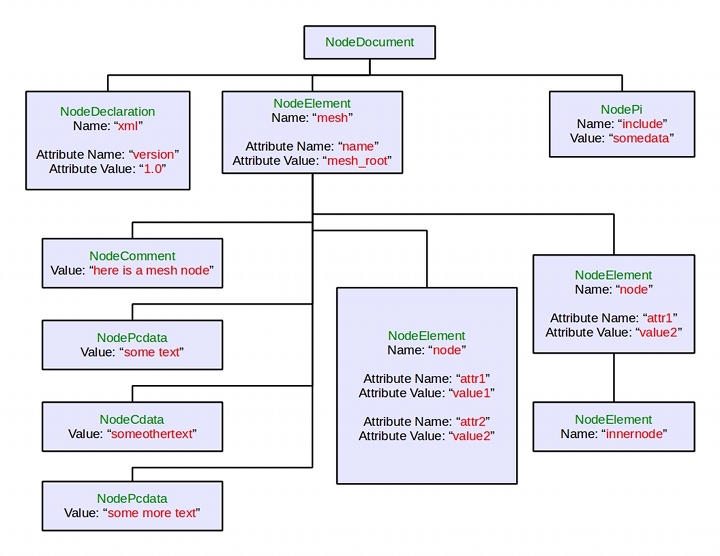
\includegraphics{SampleTree.jpg}
\caption{Complete Tree Representation of the Sample}
\end{DoxyImage}
  
\end{DoxyItemize}\hypertarget{XMLManual_XMLInterface}{}\subsubsection{C++ interface}\label{XMLManual_XMLInterface}
Despite the fact that there are several node types, there are only three C++ classes representing the tree (\hyperlink{classphys_1_1xml_1_1Document}{phys::xml::Document}, \hyperlink{classphys_1_1xml_1_1Node}{phys::xml::Node}, \hyperlink{classphys_1_1xml_1_1Attribute}{phys::xml::Attribute}); some operations on \hyperlink{classphys_1_1xml_1_1Node}{phys::xml::Node} are only valid for certain node types. The classes are described below. \par
 \par
 \hyperlink{classphys_1_1xml_1_1Document}{phys::xml::Document} is the owner of the entire document structure; it is a non-\/copyable class. The interface of \hyperlink{classphys_1_1xml_1_1Document}{phys::xml::Document} consists of loading functions ( see \hyperlink{XMLManual_XMLLoading}{Loading Documents} ), saving functions ( see \hyperlink{XMLManual_XMLSaving}{Saving Documents} ) and the entire interface of \hyperlink{classphys_1_1xml_1_1Node}{phys::xml::Node}, which allows for document inspection and/or modification. Note that while \hyperlink{classphys_1_1xml_1_1Document}{phys::xml::Document} is a sub-\/class of \hyperlink{classphys_1_1xml_1_1Node}{phys::xml::Node}, \hyperlink{classphys_1_1xml_1_1Node}{phys::xml::Node} is not a polymorphic type; the inheritance is present only to simplify usage. Alternatively you can use the \hyperlink{classphys_1_1xml_1_1Document_a93d8521e3241281e15f77cf7568d5754}{phys::xml::Document::DocumentElement} function to get the element node that's the immediate child of the document. \par
 \par
 Default constructor of \hyperlink{classphys_1_1xml_1_1Document}{phys::xml::Document} initializes the document to the tree with only a root node ( \hyperlink{classphys_1_1xml_1_1Document}{phys::xml::Document} node). You can then populate it with data using either tree modification functions or loading functions; all loading functions destroy the previous tree with all occupied memory, which puts existing node/attribute handles for this document to invalid state. If you want to destroy the previous tree, you can use the \hyperlink{classphys_1_1xml_1_1Document_a9ab556271e4a1214ecb35ba6aef9e8e4}{phys::xml::Document::Reset} function; it destroys the tree and replaces it with either an empty one or a copy of the specified document. Destructor of \hyperlink{classphys_1_1xml_1_1Document}{phys::xml::Document} also destroys the tree, thus the lifetime of the document object should exceed the lifetimes of any node/attribute handles that point to the tree. \begin{DoxyWarning}{Warning}
While technically node/attribute handles can be alive when the tree they're referring to is destroyed, calling any member function for these handles results in undefined behavior. Thus it is recommended to make sure that the document is destroyed only after all references to its nodes/attributes are destroyed.
\end{DoxyWarning}
\hyperlink{classphys_1_1xml_1_1Node}{phys::xml::Node} is the handle to a document node; it can point to any node in the document, including the document node itself. There is a common interface for nodes of all types; the actual node type can be queried via the \hyperlink{classphys_1_1xml_1_1Node_a33288f89218baf24d1061c6eeb08687f}{phys::xml::Node::Type()} method. Note that \hyperlink{classphys_1_1xml_1_1Node}{phys::xml::Node} is only a handle to the actual node, not the node itself -\/ you can have several phys::xml::node handles pointing to the same underlying object. Destroying \hyperlink{classphys_1_1xml_1_1Node}{phys::xml::Node} handle does not destroy the node and does not remove it from the tree. The size of \hyperlink{classphys_1_1xml_1_1Node}{phys::xml::Node} is equal to that of a pointer, so it is nothing more than a lightweight wrapper around a pointer; you can safely pass or return \hyperlink{namespacephys_1_1xml}{phys::xml}:Node objects by value without additional overhead. \par
 \par
 There is a special value of \hyperlink{classphys_1_1xml_1_1Node}{phys::xml::Node} type, known as null node or empty node (such nodes have type NodeNull). It does not correspond to any node in any document, and thus resembles null pointer. However, all operations are defined on empty nodes; generally the operations don't do anything and return empty nodes/attributes or empty strings as their result (see documentation for specific functions for more detailed information). This is useful for chaining calls; i.e. you can get the grandparent of a node like so: node.GetParent().GetParent(); if a node is a null node or it does not have a parent, the first Node::GetParent() call returns null node; the second GetParent() call then also returns null node, which can make error handling easier. \par
 \par
 \hyperlink{classphys_1_1xml_1_1Attribute}{phys::xml::Attribute} is a handle to an XML attribute; it has the same semantics as \hyperlink{classphys_1_1xml_1_1Node}{phys::xml::Node}, i.e. there can be several \hyperlink{classphys_1_1xml_1_1Attribute}{phys::xml::Attribute} handles pointing to the same underlying object and there is a special null attribute value, which propagates to function results. \par
 \par
 Both \hyperlink{classphys_1_1xml_1_1Node}{phys::xml::Node} and \hyperlink{classphys_1_1xml_1_1Attribute}{phys::xml::Attribute} have the default constructor which initializes them to null objects. \par
 \par
 \hyperlink{classphys_1_1xml_1_1Node}{phys::xml::Node} and \hyperlink{classphys_1_1xml_1_1Attribute}{phys::xml::Attribute} try to behave like pointers, that is, they can be compared with other objects of the same type, making it possible to use them as keys in associative containers. All handles to the same underlying object are equal, and any two handles to different underlying objects are not equal. Null handles only compare as equal to themselves. The result of relational comparison can not be reliably determined from the order of nodes in file or in any other way. Do not use relational comparison operators except for search optimization (i.e. associative container keys). \par
 \par
 If you want to use \hyperlink{classphys_1_1xml_1_1Node}{phys::xml::Node} or \hyperlink{classphys_1_1xml_1_1Attribute}{phys::xml::Attribute} objects as keys in hash-\/based associative containers, you can use the \hyperlink{classphys_1_1xml_1_1Node_a830a1833c4b4b012f1b4481e91ccb1ca}{phys::xml::Node::HashValue} or \hyperlink{classphys_1_1xml_1_1Attribute_ac0c27e07b705c41670a0903f4fe18378}{phys::xml::Attribute::HashValue} member functions. They return the hash values that are guaranteed to be the same for all handles to the same underlying object. The hash value for null handles is 0. \par
 \par
 Finally handles can be implicitly cast to boolean-\/like objects, so that you can test if the node/attribute is empty with the following code: if (node) \{ ... \} or if (!node) \{ ... \} else \{ ... \}. Alternatively you can check if a given Node/Attribute handle is null by calling the \hyperlink{classphys_1_1xml_1_1Attribute_a6d0157a562f283e9c87d1cc46b3405cc}{phys::xml::Attribute::Empty} or the \hyperlink{classphys_1_1xml_1_1Node_a22c00132e42702d16468489ff0bd01d8}{phys::xml::Node::Empty} Methods. \par
 \par
 Nodes and attributes do not exist without a document tree, so you can't create them without adding them to some document. Once underlying node/attribute objects are destroyed, the handles to those objects become invalid. While this means that destruction of the entire tree invalidates all node/attribute handles, it also means that destroying a subtree ( by calling \hyperlink{classphys_1_1xml_1_1Node_a946bb656b94c9d3a561200cd2cd3ee11}{phys::xml::Node::RemoveChild} ) or removing an attribute invalidates the corresponding handles. There is no way to check handle validity; you have to ensure correctness through external mechanisms. \par
 \par
 \hypertarget{XMLManual_XMLUnicode}{}\subsubsection{Unicode Interface}\label{XMLManual_XMLUnicode}
There are two choices of interface and internal representation when working with \hyperlink{namespacephys_1_1xml}{phys::xml} : you can either choose the UTF-\/8 (also called char) interface or UTF-\/16/32 (also called wchar\_\-t) one. The choice is controlled via XML\_\-WCHAR\_\-MODE define; you can set it via \hyperlink{xml_8h}{xml.h} or via preprocessor options beore engine compilation. If this define is set, the wchar\_\-t interface is used; otherwise (by default) the char interface is used. The exact wide character encoding is assumed to be either UTF-\/16 or UTF-\/32 and is determined based on the size of wchar\_\-t type. \begin{DoxyWarning}{Warning}
There are a few places that the reset of the engine assumes the use of the UTF-\/8/char interface. The task of integrating this cleanly is currently considered a low priority. If you use XML\_\-WCHAR\_\-MODE you will encounter bugs, they could be tiny or huge. Since we didn't test it, we assumed it doesn't work.
\end{DoxyWarning}
\begin{DoxyNote}{Note}
If the size of wchar\_\-t is 2, \hyperlink{namespacephys_1_1xml}{phys::xml} assumes UTF-\/16 encoding instead of UCS-\/2, which means that some characters are represented as two code points.
\end{DoxyNote}
All tree functions that work with strings work with either C-\/style null terminated strings or STL strings of the selected character type. For example, node name accessors look like this in char mode: 
\begin{DoxyCode}
 const char* phys::xml::Node::Name() const;
 bool phys::xml::Node::SetName(const char* value);
\end{DoxyCode}
 and like this in wchar\_\-t mode: 
\begin{DoxyCode}
 const wchar_t* phys::xml::Node::Name() const;
 bool phys::xml::Node::SetName(const wchar_t* value);
\end{DoxyCode}
 There is a special type, \hyperlink{namespacephys_1_1xml_afc87705cd1c2917d87b879715a2d8f6e}{phys::xml::char\_\-t}, that is defined as the character type and depends on the engine configuration; it will be also used in the documentation hereafter. There is also a type phys::xml::string\_\-t, which is defined as the STL string of the character type; it corresponds to std::string in char mode and to std::wstring in wchar\_\-t mode. \begin{DoxyNote}{Note}
This is one our list of items to integrate more tighlty. At some point \hyperlink{namespacephys_1_1xml_afc87705cd1c2917d87b879715a2d8f6e}{phys::xml::char\_\-t} will be replace by \hyperlink{namespacephys_a3098bae5b0a3cd16eec331f766cc562b}{phys::Character}, and phys::xml::string\_\-t will be replaced by \hyperlink{namespacephys_aa03900411993de7fbfec4789bc1d392e}{phys::String}. For now they remain Interoperable.
\end{DoxyNote}
In addition to the interface, the internal implementation changes to store XML data as \hyperlink{namespacephys_1_1xml_afc87705cd1c2917d87b879715a2d8f6e}{phys::xml::char\_\-t}; this means that these two modes have different memory usage characteristics. The conversion to \hyperlink{namespacephys_1_1xml_afc87705cd1c2917d87b879715a2d8f6e}{phys::xml::char\_\-t} upon document loading and from \hyperlink{namespacephys_1_1xml_afc87705cd1c2917d87b879715a2d8f6e}{phys::xml::char\_\-t} upon document saving happen automatically, which also carries minor performance penalty. The general advice however is to select the character mode based on usage scenario, i.e. if UTF-\/8 is inconvenient to process and most of your XML data is non-\/ASCII, wchar\_\-t mode is probably a better choice (if this is the case any patches, notifications or bugfixes that could be sent our way would help.) \par
 \par
 There are cases when you'll have to convert string data between UTF-\/8 and wchar\_\-t encodings; the following helper functions are provided for such purposes: 
\begin{DoxyCode}
 std::string AsUtf8(const wchar_t* str);
 std::wstring AsUtf8(const char* str);
\end{DoxyCode}
 Both functions accept a null-\/terminated string as an argument str, and return the converted string. AsUtf8 performs conversion from UTF-\/16/32 to UTF-\/8; AsWide performs conversion from UTF-\/8 to UTF-\/16/32. Invalid UTF sequences are silently discarded upon conversion. str has to be a valid string; passing null pointer results in undefined behavior. There are also two overloads with the same semantics which accept a string as an argument: 
\begin{DoxyCode}
 std::string AsUtf8(const std::wstring& str);
 std::wstring AsWide(const std::string& str);
\end{DoxyCode}
 \begin{DoxyNote}{Note}
Most examples in this documentation assume char interface and therefore will not compile with XML\_\-WCHAR\_\-MODE. This is done to simplify the documentation; usually the only changes you'll have to make is to pass wchar\_\-t string literals, i.e. instead of \par
 \par
 
\begin{DoxyCode}
 phys::xml::Node node = doc.GetChild("bookstore").FindChildbyAttribute("book", "i
      d", "12345"); 
\end{DoxyCode}
 \par
 \par
 you'll have to do \par
 \par
 
\begin{DoxyCode}
 phys::xml::Node node = doc.GetChild(L"bookstore").FindChildbyAttribute(L"book", 
      L"id", L"12345"); 
\end{DoxyCode}
 \par
 \par
 
\end{DoxyNote}
\hypertarget{XMLManual_XMLThreadSafety}{}\subsubsection{Thread-\/safety guarantees}\label{XMLManual_XMLThreadSafety}
Almost all functions in \hyperlink{namespacephys_1_1xml}{phys::xml} have the following thread-\/safety guarantees:
\begin{DoxyItemize}
\item It is safe to call free (non-\/member) functions from multiple threads
\item It is safe to perform concurrent read-\/only accesses to the same tree (all constant member functions do not modify the tree)
\item It is safe to perform concurrent read/write accesses, if there is only one read or write access to the single tree at a time
\end{DoxyItemize}

Concurrent modification and traversing of a single tree requires synchronization, for example via reader-\/writer lock. Modification includes altering document structure and altering individual node/attribute data, i.e. changing names/values. \par
 \par
 The only exception is \hyperlink{namespacephys_1_1xml_a2ad88e4331ac29a86c99d5e40b31f983}{phys::xml::SetMemory\_\-management\_\-functions}; it modifies global variables and as such is not thread-\/safe. Its usage policy has more restrictions, see \hyperlink{XMLManual_XMLCustomAlloc}{Custom memory allocation/deallocation functions} . \par
 \par
 \hypertarget{XMLManual_XMLExceptionSafety}{}\subsubsection{Exception guarantees}\label{XMLManual_XMLExceptionSafety}
With the exception of XPath, \hyperlink{namespacephys_1_1xml}{phys::xml} itself does not throw any exceptions. Additionally, most \hyperlink{namespacephys_1_1xml}{phys::xml} functions have a no-\/throw exception guarantee. \par
 \par
 This is not applicable to functions that operate on STL strings or IOstreams; such functions have either strong guarantee (functions that operate on strings) or basic guarantee (functions that operate on streams). Also functions that call user-\/defined callbacks (i.e. \hyperlink{classphys_1_1xml_1_1Node_a0029d08d3689c36d882ada0c0c9cf6e9}{phys::xml::Node::Traverse} or \hyperlink{classphys_1_1xml_1_1Node_ab2311cefdf1d7f4886cbebd7350d7731}{phys::xml::Node::FindNode}) do not provide any exception guarantees beyond the ones provided by the callback. \par
 \par
 If exception handling is not disabled with XML\_\-NO\_\-EXCEPTIONS define, XPath functions may throw \hyperlink{classphys_1_1xml_1_1XPathException}{phys::xml::XPathException} on parsing errors; also, XPath functions may throw std::bad\_\-alloc in low memory conditions. Still, XPath functions provide strong exception guarantee. \par
 \par
 \hypertarget{XMLManual_XMLMemory}{}\subsubsection{Memory management}\label{XMLManual_XMLMemory}
\hyperlink{namespacephys_1_1xml}{phys::xml} requests the memory needed for document storage in big chunks, and allocates document data inside those chunks. This section discusses replacing functions used for chunk allocation and internal memory management implementation. \par
 \par
 \begin{DoxyWarning}{Warning}
The \hyperlink{namespacephys_1_1xml}{phys::xml} memory system is pending tighter integration with memory management from the rest of the system. The functions and features described here should be considered deprecated and internal to the engine. It is highly likely they will be replaced without warning by a global system to allocate memory in a more efficient way.
\end{DoxyWarning}
\par
 \par
 \hypertarget{XMLManual_XMLCustomAlloc}{}\paragraph{Custom memory allocation/deallocation functions}\label{XMLManual_XMLCustomAlloc}
All memory for tree structure, tree data and XPath objects is allocated via globally specified functions, which default to malloc/free. You can set your own allocation functions with \hyperlink{namespacephys_1_1xml_a2ad88e4331ac29a86c99d5e40b31f983}{phys::xml::SetMemory\_\-management\_\-functions} function. The function interfaces are the same as that of malloc/free: 
\begin{DoxyCode}
 typedef void* (*AllocationFunction)(size_t size);
 typedef void (*deAllocationFunction)(void* ptr);
\end{DoxyCode}
 You can use the following accessor functions to change or get current memory management functions: 
\begin{DoxyCode}
 void phys::xml::SetMemory_management_functions(AllocationFunction allocate, 
      deAllocationFunction deallocate);
 AllocationFunction GetMemoryAllocationFunctionn();
 deAllocationFunction GetMemoryDeallocationFunction();
\end{DoxyCode}
 Allocation function is called with the size (in bytes) as an argument and should return a pointer to a memory block with alignment that is suitable for storage of primitive types (usually a maximum of void$\ast$ and double types alignment is sufficient) and size that is greater than or equal to the requested one. If the allocation fails, the function has to return null pointer (throwing an exception from allocation function results in undefined behavior). \par
 \par
 Deallocation function is called with the pointer that was returned by some call to allocation function; it is never called with a null pointer. If memory management functions are not thread-\/safe, library thread safety is not guaranteed. \par
 \par
 When setting new memory management functions, care must be taken to make sure that there are no live \hyperlink{namespacephys_1_1xml}{phys::xml} objects. Otherwise when the objects are destroyed, the new deallocation function will be called with the memory obtained by the old allocation function, resulting in undefined behavior. \par
 \par
 \hypertarget{XMLManual_XMLMemoryInternals}{}\paragraph{Document memory management internals}\label{XMLManual_XMLMemoryInternals}
Constructing a document object using the default constructor does not result in any allocations; document node is stored inside the \hyperlink{classphys_1_1xml_1_1Document}{phys::xml::Document} object \par
 \par
 When the document is loaded from file/buffer, unless an inplace loading function is used ( see \hyperlink{XMLManual_XMLLoadingFromMemory}{Loading document from memory} ), a complete copy of character stream is made; all names/values of nodes and attributes are allocated in this buffer. This buffer is allocated via a single large allocation and is only freed when document memory is reclaimed (i.e. if the \hyperlink{classphys_1_1xml_1_1Document}{phys::xml::Document} object is destroyed or if another document is loaded in the same object). Also when loading from file or stream, an additional large allocation may be performed if encoding conversion is required; a temporary buffer is allocated, and it is freed before load function returns. \par
 \par
 All additional memory, such as memory for document structure (node/attribute objects) and memory for node/attribute names/values is allocated in pages on the order of 32 kilobytes; actual objects are allocated inside the pages using a memory management scheme optimized for fast allocation/deallocation of many small objects. Because of the scheme specifics, the pages are only destroyed if all objects inside them are destroyed; also, generally destroying an object does not mean that subsequent object creation will reuse the same memory. This means that it is possible to devise a usage scheme which will lead to higher memory usage than expected; one example is adding a lot of nodes, and them removing all even numbered ones; not a single page is reclaimed in the process. However this is an example specifically crafted to produce unsatisfying behavior; in all practical usage scenarios the memory consumption is less than that of a general-\/purpose allocator because allocation meta-\/data is very small in size. \par
 \par
 \hypertarget{XMLManual_XMLLoading}{}\subsection{Loading Documents}\label{XMLManual_XMLLoading}

\begin{DoxyItemize}
\item \hyperlink{XMLManual_XMLLoadingFiles}{Loading Document from a File}
\item \hyperlink{XMLManual_XMLLoadingFromMemory}{Loading document from memory}
\item \hyperlink{XMLManual_XMLLoadingStreams}{Loading document from C++ IOstreams}
\item \hyperlink{XMLManual_XMLLoadingErrors}{Handling Parsing Errors}
\item \hyperlink{XMLManual_XMLLoadingParsingOptions}{Parsing Options}
\item \hyperlink{XMLManual_XMLLoadingEncodings}{Encodings}
\item \hyperlink{XMLManual_XMLLoadingStandards}{Conformance to W3C Specification}
\end{DoxyItemize}

\hyperlink{namespacephys_1_1xml}{phys::xml} provides several functions for loading XML data from various places -\/ files, C++ iostreams, memory buffers. All functions use an extremely fast non-\/validating parser. This parser is not fully W3C conformant -\/ it can load any valid XML document, but does not perform some well-\/formedness checks. While considerable effort is made to reject invalid XML documents, some validation is not performed for performance reasons. Also some XML transformations (i.e. EOL handling or attribute value normalization) can impact parsing speed and thus can be disabled. However for vast majority of XML documents there is no performance difference between different parsing options. Parsing options also control whether certain XML nodes are parsed; see \hyperlink{XMLManual_XMLLoadingParsingOptions}{Parsing Options} for more information. \par
 \par
 XML data is always converted to internal character format ( see \hyperlink{XMLManual_XMLUnicode}{Unicode Interface} ) before parsing. \hyperlink{namespacephys_1_1xml}{phys::xml} supports all popular Unicode encodings (UTF-\/8, UTF-\/16 (big and little endian), UTF-\/32 (big and little endian); UCS-\/2 is naturally supported since it's a strict subset of UTF-\/16) and handles all encoding conversions automatically. Unless explicit encoding is specified, loading functions perform automatic encoding detection based on first few characters of XML data, so in almost all cases you do not have to specify document encoding. Encoding conversion is described in more detail in \hyperlink{XMLManual_XMLLoadingEncodings}{Encodings}. \par
 \par
 \hypertarget{XMLManual_XMLLoadingFiles}{}\subsubsection{Loading Document from a File}\label{XMLManual_XMLLoadingFiles}
The most common source of XML data is files; \hyperlink{namespacephys_1_1xml}{phys::xml} provides dedicated functions for loading an XML document from \href{file:}{\tt file:} 
\begin{DoxyCode}
 phys::xml::ParseResult phys::xml::Document::LoadFile(const char* path, unsigned 
      int options = ParseDefault, phys::xml::Encoding DocumentEncoding = EncodingAuto);
      
 phys::xml::ParseResult phys::xml::Document::LoadFile(const wchar_t* path, unsign
      ed int options = ParseDefault, phys::xml::Encoding DocumentEncoding = EncodingAut
      o);
\end{DoxyCode}
 These functions accept the file path as its first argument, and also two optional arguments, which specify parsing options (see Parsing options) and input data encoding ( see \hyperlink{XMLManual_XMLLoadingEncodings}{Encodings} ). The path has the target operating system format, so it can be a relative or absolute one, it should have the delimiters of the target system, it should have the exact case if the target file system is case-\/sensitive, and is subject to any other restrictions of the underlying filesystem. \par
 \par
 File path is passed to the system file opening function as is in case of the first function (which accepts const char$\ast$ path); the second function either uses a special file opening function if it is provided by the runtime library or converts the path to UTF-\/8 and uses the system file opening function. \par
 \par
 Document::LoadFile destroys the existing document tree and then tries to load the new tree from the specified file. The result of the operation is returned in an \hyperlink{structphys_1_1xml_1_1ParseResult}{phys::xml::ParseResult} object; this object contains the operation status and the related information (i.e. last successfully parsed position in the input file, if parsing fails). See \hyperlink{XMLManual_XMLLoadingErrors}{Handling Parsing Errors} for error handling details. \par
 \par
 This is an example of loading XML document from \href{file:}{\tt file:} 
\begin{DoxyCode}
 phys::xml::Document Doc;
 phys::xml::ParseResult Result = Doc.LoadFile("tree.xml");
 std::cout << "Load result: " << Result.Description() << std::endl;
\end{DoxyCode}
 \hypertarget{XMLManual_XMLLoadingFromMemory}{}\subsubsection{Loading document from memory}\label{XMLManual_XMLLoadingFromMemory}
Sometimes XML data should be loaded from some other source than a file, i.e. HTTP URL; also you may want to load XML data from file using non-\/standard functions, i.e. to use your virtual file system facilities or to load XML from gzip-\/compressed files. All these scenarios require loading document from memory. First you should prepare a contiguous memory block with all XML data; then you have to invoke one of buffer loading functions. These functions will handle the necessary encoding conversions, if any, and then will parse the data into the corresponding XML tree. There are several buffer loading functions, which differ in the behavior and thus in performance/memory usage: 
\begin{DoxyCode}
 phys::xml::ParseResult phys::xml::Document::LoadBuffer (const void *contents, si
      ze_t size, unsigned int options=ParseDefault, Encoding DocumentEncoding=EncodingA
      uto);
 phys::xml::ParseResult phys::xml::Document::LoadBufferInplace (void *contents, s
      ize_t size, unsigned int options=ParseDefault, Encoding DocumentEncoding=Encoding
      Auto);
 phys::xml::ParseResult phys::xml::Document::LoadBufferInplaceOwn (void *contents
      , size_t size, unsigned int options=ParseDefault, Encoding DocumentEncoding=Encod
      ingAuto)
\end{DoxyCode}
 All functions accept the buffer which is represented by a pointer to XML data, contents, and data size in bytes. Also there are two optional arguments, which specify parsing options ( see \hyperlink{XMLManual_XMLLoadingParsingOptions}{Parsing Options} ) and input data encoding ( see \hyperlink{XMLManual_XMLLoadingEncodings}{Encodings} ). The buffer does not have to be zero-\/terminated. \par
 \par
 \hyperlink{classphys_1_1xml_1_1Document_a31c36783e033d6d43d51e31a6dd4099f}{phys::xml::Document::LoadBuffer} function works with immutable buffer -\/ it does not ever modify the buffer. Because of this restriction it has to create a private buffer and copy XML data to it before parsing (applying encoding conversions if necessary). This copy operation carries a performance penalty, so inplace functions are provided -\/ \hyperlink{classphys_1_1xml_1_1Document_ad1dd510bd1106edb92c69715eb015dc3}{phys::xml::Document::LoadBufferInplace} and \hyperlink{classphys_1_1xml_1_1Document_a9213b8bf4fa5423ea292a3d03c826608}{phys::xml::Document::LoadBufferInplaceOwn} store the document data in the buffer, modifying it in the process. In order for the document to stay valid, you have to make sure that the buffer's lifetime exceeds that of the tree if you're using inplace functions. In addition to that, \hyperlink{classphys_1_1xml_1_1Document_ad1dd510bd1106edb92c69715eb015dc3}{phys::xml::Document::LoadBufferInplace} does not assume ownership of the buffer, so you'll have to destroy it yourself; \hyperlink{classphys_1_1xml_1_1Document_a9213b8bf4fa5423ea292a3d03c826608}{phys::xml::Document::LoadBufferInplaceOwn} assumes ownership of the buffer and destroys it once it is not needed. This means that if you're using \hyperlink{classphys_1_1xml_1_1Document_a9213b8bf4fa5423ea292a3d03c826608}{phys::xml::Document::LoadBufferInplaceOwn}, you have to allocate memory with \hyperlink{namespacephys_1_1xml}{phys::xml} allocation function ( Not recomended, the Allocation API may be getting updates in the near future ). \par
 \par
 The best way from the performance/memory point of view is to load document using \hyperlink{classphys_1_1xml_1_1Document_a9213b8bf4fa5423ea292a3d03c826608}{phys::xml::Document::LoadBufferInplaceOwn}; this function has maximum control of the buffer with XML data so it is able to avoid redundant copies and reduce peak memory usage while parsing. However, this is not recommendeded unless you have to load the document from memory and performance is critical. Once the memory portion of the API has stabilized this will become the ideal \par
 \par
 There is also a simple helper function for cases when you want to load the XML document from null-\/terminated character string: 
\begin{DoxyCode}
 phys::xml::ParseResult phys::xml::Document::Load(const char_t *contents, unsigne
      d int options=ParseDefault);
\end{DoxyCode}
 It is equivalent to calling \hyperlink{classphys_1_1xml_1_1Document_a31c36783e033d6d43d51e31a6dd4099f}{phys::xml::Document::LoadBuffer} with size being either strlen(contents) or wcslen(contents) $\ast$ sizeof(wchar\_\-t), depending on the character type. This function assumes native encoding for input data, so it does not do any encoding conversion. In general, this function is fine for loading small documents from string literals, but has more overhead and less functionality than the buffer loading functions. \par
 \par
 This is an example of loading XML document from memory using LoadBuffer: 
\begin{DoxyCode}
 const char Source[] = "<mesh name='sphere'><bounds>0 0 1 1</bounds></mesh>";
 size_t Size = sizeof(Source);

 // You can use LoadBuffer to load the document from an immutable memory block:
 phys::xml::ParseResult Result = doc.LoadBuffer(Source, Size);
\end{DoxyCode}
 This is an example of loading XML document from memory using LoadBufferInplace: 
\begin{DoxyCode}
 const char Source[] = "<mesh name='sphere'><bounds>0 0 1 1</bounds></mesh>";
 size_t Size = sizeof(Source);

 // You can use LoadBufferInplace to load document from mutable memory block
 // the block's lifetime must exceed that of document
 char* Buffer = new char[Size];
 memcpy(Buffer, Source, Size);

 // The block can be allocated by any method; the block is modified during parsin
      g
 phys::xml::ParseResult Result = doc.LoadBufferInplace(Buffer, Size);

 // You have to destroy the block yourself after the document is no longer used
 delete[] Buffer;
\end{DoxyCode}
 This is an example of loading XML document from memory using Load and a string literal: 
\begin{DoxyCode}
 // You can use Load to load document from null-terminated strings, for example l
      iterals:
 phys::xml::ParseResult Result = doc.Load("<mesh name='sphere'><bounds>0 0 1 1</b
      ounds></mesh>");
\end{DoxyCode}
 \hypertarget{XMLManual_XMLLoadingStreams}{}\subsubsection{Loading document from C++ IOstreams}\label{XMLManual_XMLLoadingStreams}
To enhance interoperability, \hyperlink{namespacephys_1_1xml}{phys::xml} provides functions for loading document from any object which implements C++ std::istream interface. This allows you to load documents from any standard C++ stream (i.e. file stream) or any third-\/party compliant implementation (i.e. Boost Iostreams). There are two functions, one works with narrow character streams, another handles wide character ones: 
\begin{DoxyCode}
 phys::xml::ParseResult phys::xml::Document::Load (std::basic_istream< char, std:
      :char_traits< char > > &stream, unsigned int options=ParseDefault, Encoding Docum
      entEncoding=EncodingAuto);
 phys::xml::ParseResult phys::xml::Document::Load (std::basic_istream< wchar_t, s
      td::char_traits< wchar_t > > &stream, unsigned int options=ParseDefault);
\end{DoxyCode}
 \hyperlink{classphys_1_1xml_1_1Document_a9d4ddfd3b987fa3d31d41c06d06a001e}{phys::xml::Document::Load} with std::istream argument loads the document from stream from the current read position to the end, treating the stream contents as a byte stream of the specified encoding (with encoding autodetection as necessary). Thus calling \hyperlink{classphys_1_1xml_1_1Document_a9d4ddfd3b987fa3d31d41c06d06a001e}{phys::xml::Document::Load} on an opened std::ifstream object is equivalent to calling \hyperlink{classphys_1_1xml_1_1Document_a7f9dfcc3d30347773f92c8d46fe18f9a}{phys::xml::Document::LoadFile}. \par
 \par
 \hyperlink{classphys_1_1xml_1_1Document_a9d4ddfd3b987fa3d31d41c06d06a001e}{phys::xml::Document::Load} with std::wstream argument treats the stream contents as a wide character stream ( encoding is always \hyperlink{namespacephys_1_1xml_a420f5de782438f88160321385bea2015}{Encoding::Encodingwchar\_\-t} ). Because of this, using \hyperlink{classphys_1_1xml_1_1Document_a7f9dfcc3d30347773f92c8d46fe18f9a}{phys::xml::Document::LoadFile} with wide character streams requires careful (usually platform-\/specific) stream setup (i.e. using the imbue function). Generally use of wide streams is discouraged, however it provides you the ability to load documents from non-\/Unicode encodings, i.e. you can load Shift-\/JIS encoded data if you set the correct locale. \par
 \par
 This is a simple example of loading XML document from a file using streams read: 
\begin{DoxyCode}
 std::ifstream Stream("weekly-utf-8.xml");
 phys::xml::ParseResult Result = Doc.Load(Stream);
\end{DoxyCode}
 Stream loading requires working seek/tell functions and therefore may fail when used with some stream implementations like gzstream. \par
 \par
 \hypertarget{XMLManual_XMLLoadingErrors}{}\subsubsection{Handling Parsing Errors}\label{XMLManual_XMLLoadingErrors}
All document loading functions return the parsing result via \hyperlink{structphys_1_1xml_1_1ParseResult}{phys::xml::ParseResult} object. It contains parsing status, the offset of last successfully parsed character from the beginning of the source stream, and the encoding of the source stream. \par
 \par
 Parsing status is represented as the \hyperlink{namespacephys_1_1xml_ae7aabb879b21c73d8183a54470f8917f}{phys::xml::ParseStatus} enumeration and can be one of the following:
\begin{DoxyItemize}
\item \hyperlink{namespacephys_1_1xml_ae7aabb879b21c73d8183a54470f8917f}{ParseStatus::StatusOk} means that no error was encountered during parsing; the source stream represents the valid XML document which was fully parsed and converted to a tree.
\item \hyperlink{namespacephys_1_1xml_ae7aabb879b21c73d8183a54470f8917f}{ParseStatus::StatusFileNotFound} is only returned by Document::LoadFile function and means that file could not be opened.
\item \hyperlink{namespacephys_1_1xml_ae7aabb879b21c73d8183a54470f8917f}{ParseStatus::StatusIOError} is returned by Document::LoadFile function and by load functions with std::istream/std::wstream arguments; it means that some I/O error has occurred during reading the file/stream.
\item \hyperlink{namespacephys_1_1xml_ae7aabb879b21c73d8183a54470f8917f}{ParseStatus::StatusOutOfMemory} means that there was not enough memory during some allocation; any allocation failure during parsing results in this error.
\item \hyperlink{namespacephys_1_1xml_ae7aabb879b21c73d8183a54470f8917f}{ParseStatus::StatusInternalError} means that something went horribly wrong; currently this error does not occur.
\item \hyperlink{namespacephys_1_1xml_ae7aabb879b21c73d8183a54470f8917f}{ParseStatus::StatusUnrecognizedTag} means that parsing stopped due to a tag with either an empty name or a name which starts with incorrect character, such as \#.
\item \hyperlink{namespacephys_1_1xml_ae7aabb879b21c73d8183a54470f8917f}{ParseStatus::StatusBadPi} means that parsing stopped due to incorrect document declaration/processing instruction.
\item \hyperlink{namespacephys_1_1xml_ae7aabb879b21c73d8183a54470f8917f}{ParseStatus::StatusBadComment, StatusBadCdata, StatusBadDocType and StatusBadPcdata} mean that parsing stopped due to the invalid construct of the respective type
\item \hyperlink{namespacephys_1_1xml_ae7aabb879b21c73d8183a54470f8917f}{ParseStatus::StatusBadStartElement} means that parsing stopped because starting tag either had no closing $>$ symbol or contained some incorrect symbol
\item \hyperlink{namespacephys_1_1xml_ae7aabb879b21c73d8183a54470f8917f}{ParseStatus::StatusBadAttribute} means that parsing stopped because there was an incorrect attribute, such as an attribute without value or with value that is not quoted (note that $<$node attr=1$>$ is incorrect in XML)
\item \hyperlink{namespacephys_1_1xml_ae7aabb879b21c73d8183a54470f8917f}{ParseStatus::StatusBadEndElement} means that parsing stopped because ending tag had incorrect syntax (i.e. extra non-\/whitespace symbols between tag name and $>$)
\item \hyperlink{namespacephys_1_1xml_ae7aabb879b21c73d8183a54470f8917f}{ParseStatus::StatusEndElementMismatch} means that parsing stopped because the closing tag did not match the opening one (i.e. $<$node$>$$<$/nedo$>$) or because some tag was not closed at all.
\end{DoxyItemize}

\hyperlink{structphys_1_1xml_1_1ParseResult_a7f31e89fbe1735e5092adfc352ae5a0d}{phys::xml::ParseResult::Description} member function can be used to convert parsing status to a string; the returned message is always in English, so you'll have to write your own function if you need a localized string. However please note that the exact messages returned by the Description() function may change from version to version, so any complex status handling should be based on the Status value. \par
 \par
 If parsing failed because the source data was not a valid XML, the resulting tree is not destroyed -\/ despite the fact that load function returns error, you can use the part of the tree that was successfully parsed. Obviously, the last element may have an unexpected name/value; for example, if the attribute value does not end with the necessary quotation mark, like in $<$node attr=\char`\"{}value$>$some data$<$/node$>$ example, the value of attribute attr will contain the string \char`\"{}value$>$some data$<$/node$>$". \par
 \par
 In addition to the Status code, \hyperlink{structphys_1_1xml_1_1ParseResult}{phys::xml::ParseResult} has an Offset member, which contains the offset of last successfully parsed character if parsing failed because of an error in source data; otherwise offset is 0. For parsing efficiency reasons, \hyperlink{namespacephys_1_1xml}{phys::xml} does not track the current line during parsing; this offset is in units of \hyperlink{namespacephys_1_1xml_afc87705cd1c2917d87b879715a2d8f6e}{phys::xml::char\_\-t} (bytes for character mode, wide characters for wide character mode). Many text editors support 'Go To Position' feature -\/ you can use it to locate the exact error position. Alternatively, if you're loading the document from memory, you can display the error chunk along with the error description. \begin{DoxyWarning}{Warning}
Offset is calculated in the XML buffer in native encoding; if encoding conversion is performed during parsing, offset can not be used to reliably track the error position.
\end{DoxyWarning}
\hyperlink{structphys_1_1xml_1_1ParseResult}{phys::xml::ParseResult} also has a DocumentEncoding member, which can be used to check that the source data encoding was correctly guessed. It is equal to the exact encoding used during parsing (i.e. with the exact endianness); see \hyperlink{XMLManual_XMLLoadingEncodings}{Encodings} for more information. \par
 \par
 A \hyperlink{structphys_1_1xml_1_1ParseResult}{phys::xml::ParseResult} object can be implicitly converted to bool; if you do not want to handle parsing errors thoroughly, you can just check the return value of load functions as if it was a bool: if (doc.load\_\-file(\char`\"{}file.xml\char`\"{})) \{ //on Successful parse \} else \{ //on failed parse \}. A True is returned if parsing was successful. \par
 \par
 This is an example of handling loading errors: 
\begin{DoxyCode}
 const char Source[] = "<mesh name='sphere'><bounds>0 0 1 1</bounds></mesh>";
 phys::xml::Document Doc;
 phys::xml::ParseResult Result = Doc.Load(Source);

 if (Result)
     std::cout << "XML [" << Source << "] parsed without errors\n\n";
 else
 {
     std::cout << "XML [" << Source << "] parsed with errors\n";
     std::cout << "Error description: " << Result.Description() << "\n";
     std::cout << "Error offset: " << Result.Offset << " (error at [..." << (Sour
      ce + Result.Offset) << "]\n\n";
 }
\end{DoxyCode}
 \hypertarget{XMLManual_XMLLoadingParsingOptions}{}\subsubsection{Parsing Options}\label{XMLManual_XMLLoadingParsingOptions}
All document loading functions accept the optional parameter options. This is a bitmask that customizes the parsing process: you can select the node types that are parsed and various transformations that are performed with the XML text. Disabling certain transformations can improve parsing performance for some documents; however, the code for all transformations is very well optimized, and thus the majority of documents won't get any performance benefit. As a general rule, only modify parsing flags if you want to get some nodes in the document that are excluded by default (i.e. declaration or comment nodes). \begin{DoxyNote}{Note}
You should use the usual bitwise arithmetic to manipulate the bitmask: to enable a flag, use mask $|$ flag; to disable a flag, use mask \& $\sim$flag.
\end{DoxyNote}
These flags control the resulting tree contents:
\begin{DoxyItemize}
\item \hyperlink{namespacephys_1_1xml_a463f15fc43d69ab835c8598826f65646}{phys::xml::ParseDeclaration} determines if XML document declaration (node with type \hyperlink{namespacephys_1_1xml_a668b0cc666a9d49f7c7222a7552115d3}{NodeDeclaration} ) is to be put in DOM tree. If this flag is off, it is not put in the tree, but is still parsed and checked for correctness. This flag is off by default.
\item \hyperlink{namespacephys_1_1xml_adf5ee79dc4c200ad85b64a8308b0c805}{phys::xml::ParseDocType} determines if XML document type declaration (node with type \hyperlink{namespacephys_1_1xml_a668b0cc666a9d49f7c7222a7552115d3}{NodeDocType} ) is to be put in DOM tree. If this flag is off, it is not put in the tree, but is still parsed and checked for correctness. This flag is off by default.
\item \hyperlink{namespacephys_1_1xml_a4d324954fc33d50155bae04587da13e2}{phys::xml::ParsePi} determines if processing instructions (nodes with type \hyperlink{namespacephys_1_1xml_a668b0cc666a9d49f7c7222a7552115d3}{NodePi} ) are to be put in DOM tree. If this flag is off, they are not put in the tree, but are still parsed and checked for correctness. Note that \char`\"{}$<$?xml ...?$>$\char`\"{} (document declaration) is not considered to be a PI. This flag is off by default.
\item \hyperlink{namespacephys_1_1xml_a83ba30a7bee5a0fd4aa2f6136c8793fc}{phys::xml::ParseComments} determines if comments (nodes with type \hyperlink{namespacephys_1_1xml_a668b0cc666a9d49f7c7222a7552115d3}{NodeComment} ) are to be put in DOM tree. If this flag is off, they are not put in the tree, but are still parsed and checked for correctness. This flag is off by default.
\item \hyperlink{namespacephys_1_1xml_aec00a2a16700dfd76f8f3c776bd000ac}{phys::xml::ParseCdata} determines if CDATA sections (nodes with type \hyperlink{namespacephys_1_1xml_a668b0cc666a9d49f7c7222a7552115d3}{NodeCdata} ) are to be put in DOM tree. If this flag is off, they are not put in the tree, but are still parsed and checked for correctness. This flag is on by default.
\item \hyperlink{namespacephys_1_1xml_a48c0da99d1ed62b1a4984293e64828c6}{phys::xml::ParseWsPcdata} determines if PCDATA nodes (nodes with type \hyperlink{namespacephys_1_1xml_a668b0cc666a9d49f7c7222a7552115d3}{NodePcdata} ) that consist only of whitespace characters are to be put in DOM tree. Often whitespace-\/only data is not significant for the application, and the cost of allocating and storing such nodes (both memory and speed-\/wise) can be significant. For example, after parsing XML string \char`\"{}$<$node$>$ $<$a/$>$ $<$/node$>$, $<$node$>$\char`\"{} element will have three children when \hyperlink{namespacephys_1_1xml_a48c0da99d1ed62b1a4984293e64828c6}{phys::xml::ParseWsPcdata} is set (child with type \hyperlink{namespacephys_1_1xml_a668b0cc666a9d49f7c7222a7552115d3}{NodePcdata} and value \char`\"{} \char`\"{}, child with type \hyperlink{namespacephys_1_1xml_a668b0cc666a9d49f7c7222a7552115d3}{NodeElement} and name \char`\"{}a\char`\"{}, and another child with type \hyperlink{namespacephys_1_1xml_a668b0cc666a9d49f7c7222a7552115d3}{NodePcdata} and value \char`\"{} \char`\"{}), and only one child when \hyperlink{namespacephys_1_1xml_a48c0da99d1ed62b1a4984293e64828c6}{phys::xml::ParseWsPcdata} is not set. This flag is off by default.
\end{DoxyItemize}

These flags control the transformation of tree element contents:
\begin{DoxyItemize}
\item \hyperlink{namespacephys_1_1xml_a6463412ba9e404b6890e4721255cd8ed}{phys::xml::ParseEscapes} determines if character and entity references are to be expanded during the parsing process. Character references have the form \&\#...; or \&\#x...; (... is Unicode numeric representation of character in either decimal ( \&\#...; ) or hexadecimal ( \&\#x...; ) form), entity references are \&lt;, \&gt;, \&amp;, \&apos; and \&quot; (note that as \hyperlink{namespacephys_1_1xml}{phys::xml} does not handle DTD, the only allowed entities are predefined ones). If character/entity reference can not be expanded, it is left as is, so you can do additional processing later. Reference expansion is performed on attribute values and PCDATA content. This flag is on by default.
\item \hyperlink{namespacephys_1_1xml_a52af747730d2b3a313eebed4cf49a333}{phys::xml::ParseEol} determines if EOL handling (that is, replacing sequences 0x0d 0x0a by a single 0x0a character, and replacing all standalone 0x0d characters by 0x0a) is to be performed on input data (that is, comments contents, PCDATA/CDATA contents and attribute values). If this is set all $\backslash$r $\backslash$n will replaced with $\backslash$n. This flag is on by default.
\item \hyperlink{namespacephys_1_1xml_af9f7575e3cb8a0d8ad9a7ceee5e26983}{phys::xml::ParseWconvAttribute} determines if attribute value normalization should be performed for all attributes. This means, that whitespace characters (new line, tab and space) are replaced with space (' '). New line characters are always treated as if \hyperlink{namespacephys_1_1xml_a52af747730d2b3a313eebed4cf49a333}{phys::xml::ParseEol} is set, i.e. $\backslash$r $\backslash$n is converted to a single space. This flag is on by default.
\item \hyperlink{namespacephys_1_1xml_acddcc88320f06c933c67cdd77704c838}{phys::xml::ParseWnormAttribute} determines if extended attribute value normalization should be performed for all attributes. This means, that after attribute values are normalized as if \hyperlink{namespacephys_1_1xml_af9f7575e3cb8a0d8ad9a7ceee5e26983}{phys::xml::ParseWconvAttribute} was set, leading and trailing space characters are removed, and all sequences of space characters are replaced by a single space character. The value of \hyperlink{namespacephys_1_1xml_af9f7575e3cb8a0d8ad9a7ceee5e26983}{phys::xml::ParseWconvAttribute} was set has no effect if this flag is on. This flag is off by default.
\end{DoxyItemize}

\begin{DoxyNote}{Note}
\hyperlink{namespacephys_1_1xml_af9f7575e3cb8a0d8ad9a7ceee5e26983}{phys::xml::ParseWconvAttribute} option performs transformations that are required by W3C specification for attributes that are declared as CDATA; ParseWnormAttribute performs transformations required for NMTOKENS attributes. In the absence of document type declaration all attributes should behave as if they are declared as CDATA, thus \hyperlink{namespacephys_1_1xml_af9f7575e3cb8a0d8ad9a7ceee5e26983}{phys::xml::ParseWconvAttribute} is the default option.
\end{DoxyNote}
Additionally there are three predefined option masks:
\begin{DoxyItemize}
\item \hyperlink{namespacephys_1_1xml_ab660837afbc6aaab22425d8d23e8f2e4}{phys::xml::ParseMinimal} has all options turned off. This option mask means that \hyperlink{namespacephys_1_1xml}{phys::xml} does not add declaration nodes, document type declaration nodes, PI nodes, CDATA sections and comments to the resulting tree and does not perform any conversion for input data, so theoretically it is the fastest mode. However, as mentioned above, in practice \hyperlink{namespacephys_1_1xml_aa6b8f7f8c2322fd683a235b498834d60}{phys::xml::ParseDefault} is usually equally fast.
\item \hyperlink{namespacephys_1_1xml_aa6b8f7f8c2322fd683a235b498834d60}{phys::xml::ParseDefault} is the default set of flags, i.e. it has all options set to their default values. It includes parsing CDATA sections (comments/PIs are not parsed), performing character and entity reference expansion, replacing whitespace characters with spaces in attribute values and performing EOL handling. Note, that PCDATA sections consisting only of whitespace characters are not parsed (by default) for performance reasons.
\item \hyperlink{namespacephys_1_1xml_af1c356f1eb063a63efebd6c8a5241c63}{phys::xml::ParseFull} is the set of flags which adds nodes of all types to the resulting tree and performs default conversions for input data. It includes parsing CDATA sections, comments, PI nodes, document declaration node and document type declaration node, performing character and entity reference expansion, replacing whitespace characters with spaces in attribute values and performing EOL handling. Note, that PCDATA sections consisting only of whitespace characters are not parsed in this mode.
\end{DoxyItemize}

This is an example of using different parsing options: 
\begin{DoxyCode}
 const char* Source = "<!--comment--><node>&lt;</node>";

  // Parsing with default options; note that comment node is not added to the tre
      e, and entity reference &lt; is expanded
 Doc.Load(Source);
 std::cout << "First node value: [" << Doc.GetFirstChild().Value() << "], node ch
      ild value: [" << Doc.ChildValue("node") << "]\n";

 // Parsing with additional value option; comment node is now added to the tree
 Doc.Load(Source, phys::xml::ParseDefault | phys::xml::ParseComments);
 std::cout << "First node value: [" << Doc.GetFirstChild().Value() << "], node ch
      ild value: [" << Doc.ChildValue("node") << "]\n";

 // Parsing with additional value option and without the (default) parse_escapes 
      option; &lt; is not expanded
 Doc.Load(Source, (phys::xml::ParseDefault | phys::xml::ParseComments) & ~
      phys::xml::ParseEscapes);
 std::cout << "First node value: [" << Doc.GetFirstChild().Value() << "], node ch
      ild value: [" << Doc.ChildValue("node") << "]\n";

 // Parsing with minimal option mask; comment node is not added to the tree, and 
      &lt; is not expanded
 Doc.Load(Source, phys::xml::ParseMinimal);
 std::cout << "First node value: [" << Doc.GetFirstChild().Value() << "], node ch
      ild value: [" << Doc.ChildValue("node") << "]\n";
\end{DoxyCode}
 \hypertarget{XMLManual_XMLLoadingEncodings}{}\subsubsection{Encodings}\label{XMLManual_XMLLoadingEncodings}
\hyperlink{namespacephys_1_1xml}{phys::xml} supports all popular Unicode encodings (UTF-\/8, UTF-\/16 (big and little endian), UTF-\/32 (big and little endian); UCS-\/2 is naturally supported since it's a strict subset of UTF-\/16) and handles all encoding conversions. Most loading functions accept the optional parameter encoding. This is a value of enumeration type \hyperlink{namespacephys_1_1xml_a420f5de782438f88160321385bea2015}{phys::xml::Encoding}, that can have the following values:
\begin{DoxyItemize}
\item \hyperlink{namespacephys_1_1xml_a420f5de782438f88160321385bea2015}{Encoding::EncodingAuto} means that pugixml will try to guess the encoding based on source XML data. The algorithm is a modified version of the one presented in Appendix F.1 of XML recommendation; it tries to match the first few bytes of input data with the following patterns in strict order:
\begin{DoxyItemize}
\item If first four bytes match UTF-\/32 BOM (Byte Order Mark), encoding is assumed to be UTF-\/32 with the endianness equal to that of BOM;
\item If first two bytes match UTF-\/16 BOM, encoding is assumed to be UTF-\/16 with the endianness equal to that of BOM;
\item If first three bytes match UTF-\/8 BOM, encoding is assumed to be UTF-\/8;
\item If first four bytes match UTF-\/32 representation of $<$, encoding is assumed to be UTF-\/32 with the corresponding endianness;
\item If first four bytes match UTF-\/16 representation of $<$?, encoding is assumed to be UTF-\/16 with the corresponding endianness;
\item If first two bytes match UTF-\/16 representation of $<$, encoding is assumed to be UTF-\/16 with the corresponding endianness (this guess may yield incorrect result, but it's better than UTF-\/8);
\item Otherwise encoding is assumed to be UTF-\/8.
\end{DoxyItemize}
\item \hyperlink{namespacephys_1_1xml_a420f5de782438f88160321385bea2015}{Encoding::EncodingUTF8} corresponds to UTF-\/8 encoding as defined in the Unicode standard; UTF-\/8 sequences with length equal to 5 or 6 are not standard and are rejected.
\item \hyperlink{namespacephys_1_1xml_a420f5de782438f88160321385bea2015}{Encoding::EncodingUTF16LE} corresponds to little-\/endian UTF-\/16 encoding as defined in the Unicode standard; surrogate pairs are supported.
\item \hyperlink{namespacephys_1_1xml_a420f5de782438f88160321385bea2015}{Encoding::EncodingUTF16BE} corresponds to big-\/endian UTF-\/16 encoding as defined in the Unicode standard; surrogate pairs are supported.
\item \hyperlink{namespacephys_1_1xml_a420f5de782438f88160321385bea2015}{Encoding::EncodingUTF16} corresponds to UTF-\/16 encoding as defined in the Unicode standard; the endianness is assumed to be that of the target platform.
\item \hyperlink{namespacephys_1_1xml_a420f5de782438f88160321385bea2015}{Encoding::EncodingUTF32LE} corresponds to little-\/endian UTF-\/32 encoding as defined in the Unicode standard.
\item \hyperlink{namespacephys_1_1xml_a420f5de782438f88160321385bea2015}{Encoding::EncodingUTF32BE} corresponds to big-\/endian UTF-\/32 encoding as defined in the Unicode standard.
\item \hyperlink{namespacephys_1_1xml_a420f5de782438f88160321385bea2015}{Encoding::EncodingUTF32} corresponds to UTF-\/32 encoding as defined in the Unicode standard; the endianness is assumed to be that of the target platform.
\item \hyperlink{namespacephys_1_1xml_a420f5de782438f88160321385bea2015}{Encoding::Encodingwchar\_\-t } corresponds to the encoding of phys::xml::wchar\_\-t type; it has the same meaning as either \hyperlink{namespacephys_1_1xml_a420f5de782438f88160321385bea2015}{EncodingUTF16} or \hyperlink{namespacephys_1_1xml_a420f5de782438f88160321385bea2015}{EncodingUTF32}, depending on phys::xml::wchar\_\-t size.
\end{DoxyItemize}

The algorithm used for \hyperlink{namespacephys_1_1xml_a420f5de782438f88160321385bea2015}{EncodingAuto} correctly detects any supported Unicode encoding for all well-\/formed XML documents (since they start with document declaration) and for all other XML documents that start with $<$; if your XML document does not start with $<$ and has encoding that is different from UTF-\/8, use the specific encoding. \begin{DoxyNote}{Note}
The current behavior for Unicode conversion is to skip all invalid UTF sequences during conversion. This behavior should not be relied upon; moreover, in case no encoding conversion is performed, the invalid sequences are not removed, so you'll get them as is in node/attribute contents.
\end{DoxyNote}
\hypertarget{XMLManual_XMLLoadingStandards}{}\subsubsection{Conformance to W3C Specification}\label{XMLManual_XMLLoadingStandards}
\hyperlink{namespacephys_1_1xml}{phys::xml} is not fully W3C conformant -\/ it can load any valid XML document, but does not perform some well-\/formedness checks. While considerable effort is made to reject invalid XML documents, some validation is not performed because of performance reasons. \par
 \par
 There is only one non-\/conformant behavior when dealing with valid XML documents, \hyperlink{namespacephys_1_1xml}{phys::xml} does not use information supplied in document type declaration for parsing. This means that entities declared in DOCTYPE are not expanded, and all attribute/PCDATA values are always processed in a uniform way that depends only on parsing options. \par
 \par
 As for rejecting invalid XML documents, there are a number of incompatibilities with W3C specification, including:
\begin{DoxyItemize}
\item Multiple attributes of the same node can have equal names.
\item All non-\/ASCII characters are treated in the same way as symbols of English alphabet, so some invalid tag names are not rejected.
\item Attribute values which contain $<$ are not rejected.
\item Invalid entity/character references are not rejected and are instead left as is.
\item Comment values can contain -\/-\/.
\item XML data is not required to begin with document declaration; additionally, document declaration can appear after comments and other nodes.
\item Invalid document type declarations are silently ignored in some cases.
\end{DoxyItemize}\hypertarget{XMLManual_XMLAccessing}{}\subsection{Accessing Document Data}\label{XMLManual_XMLAccessing}

\begin{DoxyItemize}
\item \hyperlink{XMLManual_XMLAccessingBasics}{Basic traversal functions}
\item \hyperlink{XMLManual_XMLAccessingNodeData}{Getting Node Data}
\item \hyperlink{XMLManual_XMLAccessingAttributeData}{Getting attribute data}
\item \hyperlink{XMLManual_XMLAccessingContentBased}{Content Based Traversal Functions}
\item \hyperlink{XMLManual_XMLAccessingIterators}{Traversing Node/Attribute Lists via Iterators}
\item \hyperlink{XMLManual_XMLAccessingWalker}{Recursive traversal with phys::xml::TreeWalker}
\item \hyperlink{XMLManual_XMLAccessingPredicates}{Searching for Nodes/Attributes with Predicates}
\item \hyperlink{XMLManual_XMLAccessingMisc}{Miscellaneous functions}
\end{DoxyItemize}

\hyperlink{namespacephys_1_1xml}{phys::xml} features an extensive interface for getting various types of data from the document and for traversing the document. This section provides documentation for all such functions that do not modify the tree except for XPath-\/related functions; see \hyperlink{XMLManual_XMLXPath}{XPath} for XPath reference. As discussed in \hyperlink{XMLManual_XMLInterface}{C++ interface}, there are two types of handles to tree data -\/ \hyperlink{classphys_1_1xml_1_1Node}{phys::xml::Node} and \hyperlink{classphys_1_1xml_1_1Attribute}{phys::xml::Attribute}. The handles have special null (empty) values which propagate through various functions and thus are useful for writing more concise code; see \hyperlink{XMLManual_XMLInterface}{C++ interface} for details. The documentation in this section will explicitly state the results of all function in case of null inputs. \hypertarget{XMLManual_XMLAccessingBasics}{}\subsubsection{Basic traversal functions}\label{XMLManual_XMLAccessingBasics}
The internal representation of the document is a tree, where each node has a list of child nodes (the order of children corresponds to their order in the XML representation), additionally element nodes have a list of attributes, which is also ordered. Several functions are provided in order to let you get from one node in the tree to the other. These functions roughly correspond to the internal representation, and thus are usually building blocks for other methods of traversing (i.e. XPath traversals are based on these functions). 
\begin{DoxyCode}
 phys::xml::Node phys::xml::Node::GetParent() const;
 phys::xml::Node phys::xml::Node::GetFirstChild() const;
 phys::xml::Node phys::xml::Node::GetLastChild() const;
 phys::xml::Node phys::xml::Node::GetNextSibling() const;
 phys::xml::Node phys::xml::Node::GetPreviousSibling() const;

 phys::xml::Attribute phys::xml::Node::GetFirstAttribute() const;
 phys::xml::Attribute phys::xml::Node::GetLastAttribute() const;
 phys::xml::Attribute phys::xml::Attribute::GetNextAttribute() const;
 phys::xml::Attribute phys::xml::Attribute::GetPreviousAttribute() const;
\end{DoxyCode}
 The GetParent function returns the node's parent; all non-\/null nodes except the document have non-\/null parent. GetFirstChild and GetLastChild return the first and last child of the node, respectively; note that only document nodes and element nodes can have non-\/empty child node list. If node has no children, both functions return null nodes. GetNextSibling and GetPreviousSibling return the node that's immediately to the right/left of this node in the children list, respectively -\/ for example, in $<$a/$>$ $<$b/$>$ $<$c/$>$, calling GetNextSibling for a handle that points to $<$b/$>$ results in a handle pointing to $<$c/$>$, and calling GetPreviousSibling results in handle pointing to $<$a/$>$. If node does not have next/previous sibling (this happens if it is the last/first node in the list, respectively), the functions return null nodes. GetFirstAttribute, GetLastAttribute, GetNextAttribute and GetPreviousAttribute functions behave similarly to the corresponding child node functions and allow to iterate through attribute list in the same way. \begin{DoxyNote}{Note}
Because of memory consumption reasons, attributes do not have a link to their parent nodes. Thus there is no phys::xml::attribute::parent() function.
\end{DoxyNote}
Calling any of the functions above on the null handle results in a null handle -\/ i.e. node.GetFirstChild().GetNextSibling() returns the second child of node, and null handle if node is null, has no children at all or if it has only one child node. \par
 \par
 With these functions, you can iterate through all child nodes and display all attributes like this: 
\begin{DoxyCode}
 for (phys::xml::Node tool = tools.GetFirstChild(); tool; tool = tool.GetNextSibl
      ing())
 {
     std::cout << "Tool:";

     for (phys::xml::Attribute attr = tool.GetFirstAttribute(); attr; attr = attr
      .GetNextAttribute())
     {
         std::cout << " " << attr.Name() << "=" << attr.Value();
     }

     std::cout << std::endl;
 }
\end{DoxyCode}
 \hypertarget{XMLManual_XMLAccessingNodeData}{}\subsubsection{Getting Node Data}\label{XMLManual_XMLAccessingNodeData}
Apart from structural information (parent, child nodes, attributes), nodes can have name and value, both of which are strings. Depending on node type, name or value may be absent. \hyperlink{namespacephys_1_1xml_a668b0cc666a9d49f7c7222a7552115d3}{NodeDocument} nodes do not have a name or value, \hyperlink{namespacephys_1_1xml_a668b0cc666a9d49f7c7222a7552115d3}{NodeElement} and \hyperlink{namespacephys_1_1xml_a668b0cc666a9d49f7c7222a7552115d3}{NodeType::NodeDeclaration} nodes always have a name but never have a value, \hyperlink{namespacephys_1_1xml_a668b0cc666a9d49f7c7222a7552115d3}{NodeType::NodePcdata}, \hyperlink{namespacephys_1_1xml_a668b0cc666a9d49f7c7222a7552115d3}{NodeType::NodeCdata}, \hyperlink{namespacephys_1_1xml_a668b0cc666a9d49f7c7222a7552115d3}{NodeType::NodeComment} and \hyperlink{namespacephys_1_1xml_a668b0cc666a9d49f7c7222a7552115d3}{NodeType::NodeDocType} nodes never have a name but always have a value (it may be empty though), \hyperlink{namespacephys_1_1xml_a668b0cc666a9d49f7c7222a7552115d3}{NodeType::NodePi} nodes always have a name and a value (again, value may be empty). In order to get node's name or value, you can use the following functions: 
\begin{DoxyCode}
 const char_t* phys::xml::Node::Name() const;
 const char_t* phys::xml::Node::Value() const;
\end{DoxyCode}
 In case node does not have a name or value or if the node handle is null, both functions return empty strings -\/ they never return null pointers. \par
 \par
 It is common to store data as text contents of some node -\/ i.e. $<$node$>$ $<$description$>$ This is a node $<$/description$>$ $<$/node$>$. In this case, $<$description$>$ node does not have a value, but instead has a child of type \hyperlink{namespacephys_1_1xml_a668b0cc666a9d49f7c7222a7552115d3}{NodeType::NodePcdata} with value \char`\"{}This is a node\char`\"{}. \hyperlink{namespacephys_1_1xml}{phys::xml} provides two helper functions to parse such data: 
\begin{DoxyCode}
 const char_t* phys::xml::Node::ChildValue() const;
 const char_t* phys::xml::Node::ChildValue(const char_t* name) const;
\end{DoxyCode}
 ChildValue() returns the value of the first child with type \hyperlink{namespacephys_1_1xml_a668b0cc666a9d49f7c7222a7552115d3}{NodeType::NodePcdata} or \hyperlink{namespacephys_1_1xml_a668b0cc666a9d49f7c7222a7552115d3}{NodeType::NodeCdata}; ChildValue(Name) is a simple wrapper for Child(Name).ChildValue(). For the above example, calling node.ChildValue(\char`\"{}description\char`\"{}) and description.ChildValue() will both produce string \char`\"{}This is a node\char`\"{}. If there is no child with relevant type, or if the handle is null, ChildValue functions return empty string. \par
 \par
 There is an example of using some of these functions \hyperlink{XMLManual_XMLAccessingAttributeData}{at the end of the next section}. \hypertarget{XMLManual_XMLAccessingAttributeData}{}\subsubsection{Getting attribute data}\label{XMLManual_XMLAccessingAttributeData}
All attributes have name and value, both of which are strings (value may be empty). There are two corresponding accessors: 
\begin{DoxyCode}
 const char_t* phys::xml::Attribute::Name() const;
 const char_t* phys::xml::Attribute::Value() const;
\end{DoxyCode}
 In case the attribute handle is null, both functions return empty strings -\/ they never return null pointers. \par
 \par
 In many cases attribute values have types that are not strings -\/ i.e. an attribute may always contain values that should be treated as integers, despite the fact that they are represented as strings in XML. \hyperlink{namespacephys_1_1xml}{phys::xml} provides several accessors that convert attribute value to some other type: 
\begin{DoxyCode}
 // Native C++ types
 bool phys::xml::Attribute::AsBool() const;
 double phys::xml::Attribute::AsDouble() const;
 float phys::xml::Attribute::AsFloat() const;
 int phys::xml::Attribute::AsInt() const;
 unsigned int phys::xml::Attribute::AsUint() const;

 //Physgame abstracted types
 Real phys::xml::Attribute::AsReal() const;
 String phys::xml::Attribute::AsString() const;
 Whole phys::xml::Attribute::AsWhole() const;
\end{DoxyCode}
 AsDouble, AsFloat, AsInt, AsUint, AsReal and AsWhole convert attribute values to numbers. If attribute handle is null or attribute value is empty, 0 is returned. Otherwise, all leading whitespace characters are truncated, and the remaining string is parsed as a decimal number (AsInt, AsUint or AsWhole) or as a floating point number in either decimal or scientific form (AsDouble, AsFloat or AsReal). Any extra characters are silently discarded, i.e. AsInt will return 1 for string \char`\"{}1abc\char`\"{}. \par
 \par
 In case the input string contains a number that is out of the target numeric range, the result is undefined. \begin{DoxyWarning}{Warning}
Some number conversion functions depend on current C locale as set with setlocale, so may return unexpected results if the locale is different from \char`\"{}C\char`\"{}.
\end{DoxyWarning}
AsBool converts attribute value to boolean as follows: if attribute handle is null or attribute value is empty, false is returned. Otherwise, true is returned if the first character is one of '1', 't', 'T', 'y', 'Y'. This means that strings like \char`\"{}true\char`\"{} and \char`\"{}yes\char`\"{} are recognized as true, while strings like \char`\"{}false\char`\"{} and \char`\"{}no\char`\"{} are recognized as false. For more complex matching you'll have to write your own function. \begin{DoxyNote}{Note}
There are no portable 64-\/bit types in C++, so there is no corresponding conversion function. If your platform has a 64-\/bit integer, you can easily write a conversion function yourself. We are planning on addressing this with a new Physgame abstracted type, but we have not done so yet.
\end{DoxyNote}
This is an example of using these functions, along with node data retrieval ones: 
\begin{DoxyCode}
 for (phys::xml::Node tool = tools.GetChild("Tool"); tool; tool = tool.GetNextSib
      ling("Tool"))
 {
     std::cout << "Tool " << tool.GetAttribute("Filename").Value();
     std::cout << ": AllowRemote " << tool.GetAttribute("AllowRemote").AsBool();
     std::cout << ", Timeout " << tool.GetAttribute("Timeout").AsInt();
     std::cout << ", Description '" << tool.ChildValue("Description") << "'\n";
 }
\end{DoxyCode}
 \hypertarget{XMLManual_XMLAccessingContentBased}{}\subsubsection{Content Based Traversal Functions}\label{XMLManual_XMLAccessingContentBased}
Since a lot of document traversal consists of finding the node/attribute with the correct name, there are special functions for that purpose: 
\begin{DoxyCode}
 phys::xml::Node phys::xml::Node::GetChild(const char_t* name) const;
 phys::xml::Attribute phys::xml::Node::GetAttribute(const char_t* name) const;
 phys::xml::Node phys::xml::Node::GetNextSibling(const char_t* name) const;
 phys::xml::Node phys::xml::Node::GetPreviousSibling(const char_t* name) const;
\end{DoxyCode}
 GetChild and GetAttribute return the first child/attribute with the specified name; GetNextSibling and GetPreviousSibling return the first sibling in the corresponding direction with the specified name. All string comparisons are case-\/sensitive. In case the node handle is null or there is no node/attribute with the specified name, null handle is returned. \par
 \par
 GetChild and GetNextSibling functions can be used together to loop through all child nodes with the desired name like this: 
\begin{DoxyCode}
 for (phys::xml::Node tool = tools.GetChild("Tool"); tool; tool = tool.GetNextSib
      ling("Tool"))
     {}
\end{DoxyCode}
 Occasionally the needed node is specified not by the unique name but instead by the value of some attribute; for example, it is common to have node collections with each node having a unique id: $<$group$>$ $<$item id=\char`\"{}1\char`\"{}/$>$ $<$item id=\char`\"{}2\char`\"{}/$>$ $<$/group$>$. There are two functions for finding child nodes based on the attribute values: 
\begin{DoxyCode}
 phys::xml::Node phys::xml::Node::FindChildbyAttribute(const char_t* name, const 
      char_t* attr_name, const char_t* attr_value) const;
 phys::xml::Node phys::xml::Node::FindChildbyAttribute(const char_t* attr_name, c
      onst char_t* attr_value) const;
\end{DoxyCode}
 The three-\/argument function returns the first child node with the specified name which has an attribute with the specified name/value; the two-\/argument function skips the name test for the node, which can be useful for searching in heterogeneous collections. If the node handle is null or if no node is found, null handle is returned. All string comparisons are case-\/sensitive. \par
 \par
 In all of the above functions, all arguments have to be valid strings; passing null pointers results in undefined behavior.

This is an example of using these functions: 
\begin{DoxyCode}
 std::cout << "Tool for *.dae generation: " << tools.FindChildbyAttribute("Tool",
       "OutputFileMasks", "*.dae").GetAttribute("Filename").Value() << "\n";

 for (phys::xml::Node tool = tools.GetChild("Tool"); tool; tool = tool.GetNextSib
      ling("Tool"))
 {
     std::cout << "Tool " << tool.GetAttribute("Filename").Value() << "\n";
 }
\end{DoxyCode}
 \hypertarget{XMLManual_XMLAccessingIterators}{}\subsubsection{Traversing Node/Attribute Lists via Iterators}\label{XMLManual_XMLAccessingIterators}
Child node lists and attribute lists are simply double-\/linked lists; while you can use GetPreviousSibling/GetNextSibling and other such functions for iteration, \hyperlink{namespacephys_1_1xml}{phys::xml} additionally provides node and attribute iterators, so that you can treat nodes as containers of other nodes or attributes: 
\begin{DoxyCode}
 class phys::xml::NodeIterator;
 class phys::xml::AttributeIterator;

 typedef phys::xml::NodeIterator phys::xml::Node::iterator;
 iterator phys::xml::Node::begin() const;
 iterator phys::xml::Node::end() const;

 typedef phys::xml::AttributeIterator phys::xml::Node::attribute_iterator;
 attribute_iterator phys::xml::Node::attributes_begin() const;
 attribute_iterator phys::xml::Node::attributes_end() const;
\end{DoxyCode}
 begin and attributes\_\-begin return iterators that point to the first node/attribute, respectively; end and attributes\_\-end return past-\/the-\/end iterator for node/attribute list, respectively -\/ this iterator can't be dereferenced, but decrementing it results in an iterator pointing to the last element in the list (except for empty lists, where decrementing past-\/the-\/end iterator results in undefined behavior). Past-\/the-\/end iterator is commonly used as a termination value for iteration loops (see sample below). If you want to get an iterator that points to an existing handle, you can construct the iterator with the handle as a single constructor argument, like so: phys::xml::NodeIterator(node). For \hyperlink{classphys_1_1xml_1_1AttributeIterator}{phys::xml::AttributeIterator}, you'll have to provide both an attribute and its parent node. \par
 \par
 begin and end return equal iterators if called on null node; such iterators can't be dereferenced. attributes\_\-begin and attributes\_\-end behave the same way. For correct iterator usage this means that child node/attribute collections of null nodes appear to be empty. \begin{DoxyNote}{Note}
The names begin, end, attribute\_\-begin and attribute\_\-end were chosen for maximum compatibility. Some template functions that act on containers rely on the name begin and end. We may develop a naming scheme that fits better into the existing API in the future.
\end{DoxyNote}
Both types of iterators have bidirectional iterator semantics (i.e. they can be incremented and decremented, but efficient random access is not supported) and support all usual iterator operations -\/ comparison, dereference, etc. The iterators are invalidated if the node/attribute objects they're pointing to are removed from the tree; adding nodes/attributes does not invalidate any iterators. \par
 \par
 Here is an example of using iterators for document traversal: 
\begin{DoxyCode}
 for (phys::xml::NodeIterator it = tools.begin(); it != tools.end(); ++it)
 {
     std::cout << "Tool:";

     for (phys::xml::AttributeIterator ait = it->attributes_begin(); ait != it->a
      ttributes_end(); ++ait)
     {
         std::cout << " " << ait->Name() << "=" << ait->Value();
     }

     std::cout << std::endl;
 }
\end{DoxyCode}
 \begin{DoxyWarning}{Warning}
Node and attribute iterators are somewhere in the middle between const and non-\/const iterators. While dereference operation yields a non-\/constant reference to the object, so that you can use it for tree modification operations, modifying this reference by assignment -\/ i.e. passing iterators to a function like std::sort -\/ will not give expected results, as assignment modifies local handle that's stored in the iterator.
\end{DoxyWarning}
\hypertarget{XMLManual_XMLAccessingWalker}{}\subsubsection{Recursive traversal with phys::xml::TreeWalker}\label{XMLManual_XMLAccessingWalker}
The methods described above allow traversal of immediate children of some node; if you want to do a deep tree traversal, you'll have to do it via a recursive function or some equivalent method. However, pugixml provides a helper for depth-\/first traversal of a subtree. In order to use it, you have to implement the \hyperlink{classphys_1_1xml_1_1TreeWalker}{phys::xml::TreeWalker} interface and to call the \hyperlink{classphys_1_1xml_1_1Node_a0029d08d3689c36d882ada0c0c9cf6e9}{phys::xml::Node::Traverse} function. 
\begin{DoxyCode}
 bool phys::xml::Node::Traverse(phys::xml::TreeWalker& walker);
\end{DoxyCode}
 The traversal is launched by calling traverse function on traversal root and proceeds as follows:
\begin{DoxyItemize}
\item First, TreeWalker::begin function is called with traversal root as its argument.
\item Then, TreeWalker::for\_\-each function is called for all nodes in the traversal subtree in depth first order, excluding the traversal root. Node is passed as an argument.
\item Finally, TreeWalker::end function is called with traversal root as its argument.
\end{DoxyItemize}

\begin{DoxyWarning}{Warning}
The Names of the Treewalker could change without notice prior to the initial of the engine.
\end{DoxyWarning}
If begin, end or any of the for\_\-each calls return false, the traversal is terminated and false is returned as the traversal result; otherwise, the traversal results in true. Note that you don't have to override begin or end functions; their default implementations return true. \par
 \par
 You can get the node's depth relative to the traversal root at any point by calling TreeWalker::Depth function. It returns -\/1 if called from begin/end, and returns 0-\/based depth if called from TreeWalker::for\_\-each -\/ depth is 0 for all children of the traversal root, 1 for all grandchildren and so on. \par
 \par
 This is an example of traversing tree hierarchy with \hyperlink{classphys_1_1xml_1_1TreeWalker}{phys::xml::TreeWalker}: 
\begin{DoxyCode}
 struct SimpleWalker: phys::xml::TreeWalker
 {
     virtual bool for_each(phys::xml::Node& node)
     {
         for (int i = 0; i < Depth(); ++i) std::cout << "  "; // indentation

         std::cout << ": Name='" << node.Name() << "', Value='" << node.Value() <
      < "'\n";

         return true; // continue traversal
     }
 };
\end{DoxyCode}
 
\begin{DoxyCode}
 SimpleWalker walker;
 Doc.Traverse(walker);
\end{DoxyCode}
 \hypertarget{XMLManual_XMLAccessingPredicates}{}\subsubsection{Searching for Nodes/Attributes with Predicates}\label{XMLManual_XMLAccessingPredicates}
While there are existing functions for getting a node/attribute with known contents, they are often not sufficient for simple queries. As an alternative for manual iteration through nodes/attributes until the needed one is found, you can make a predicate and call one of Find functions: 
\begin{DoxyCode}
 template <typename Predicate> phys::xml::Attribute 
      phys::xml::Node::FindAttribute(Predicate pred) const;
 template <typename Predicate> phys::xml::Node phys::xml::Node::FindChild(Predica
      te pred) const;
 template <typename Predicate> phys::xml::Node phys::xml::Node::FindNode(Predicat
      e pred) const;
\end{DoxyCode}
 The predicate should be either a plain function or a function object which accepts one argument of type \hyperlink{classphys_1_1xml_1_1Attribute}{phys::xml::Attribute} (for FindAttribute) or \hyperlink{classphys_1_1xml_1_1Node}{phys::xml::Node} (for FindChild and FindNode), and returns bool. The predicate is never called with null handle as an argument. \par
 \par
 \hyperlink{classphys_1_1xml_1_1Node_ab1ad6ee2e78ddd3f591faffe675ed910}{phys::xml::Node::FindAttribute} function iterates through all attributes of the specified node, and returns the first attribute for which the predicate returned true. If the predicate returned false for all attributes or if there were no attributes (including the case where the node is null), null attribute is returned. \par
 \par
 \hyperlink{classphys_1_1xml_1_1Node_a1041d264f8927adb691c47ccacff28d4}{phys::xml::Node::FindChild} function iterates through all child nodes of the specified node, and returns the first node for which the predicate returned true. If the predicate returned false for all nodes or if there were no child nodes (including the case where the node is null), null node is returned. \par
 \par
 \hyperlink{classphys_1_1xml_1_1Node_ab2311cefdf1d7f4886cbebd7350d7731}{phys::xml::Node::FindNode} function performs a depth-\/first traversal through the subtree of the specified node (excluding the node itself), and returns the first node for which the predicate returned true. If the predicate returned false for all nodes or if subtree was empty, null node is returned. \par
 \par
 Here are some sample predicates: 
\begin{DoxyCode}
 bool SmallTimeout(phys::xml::Node node)
 {
     return node.GetAttribute("Timeout").AsInt() < 20;
 }

 struct AllowRemotePredicate
 {
     bool operator()(phys::xml::Attribute attr) const
     {
         return strcmp(attr.Name(), "AllowRemote") == 0;
     }

     bool operator()(phys::xml::Node node) const
     {
         return node.GetAttribute("AllowRemote").AsBool();
     }
 };
\end{DoxyCode}
 This is an example of using predicate-\/based functions: 
\begin{DoxyCode}
 // Find child via predicate (looks for direct children only)
 std::cout << tools.FindChild(AllowRemotePredicate()).GetAttribute("Filename").Va
      lue() << std::endl;

 // Find node via predicate (looks for all descendants in depth-first order)
 std::cout << doc.FindNode(AllowRemotePredicate()).GetAttribute("Filename").Value
      () << std::endl;

 // Find attribute via predicate
 std::cout << tools.LastChild().FindAttribute(AllowRemotePredicate()).Value() << 
      std::endl;

 // We can use simple functions instead of function objects
 std::cout << tools.FindChild(SmallTimeout).GetAttribute("Filename").Value() << s
      td::endl;
\end{DoxyCode}
 \hypertarget{XMLManual_XMLAccessingMisc}{}\subsubsection{Miscellaneous functions}\label{XMLManual_XMLAccessingMisc}
If you need to get the document root of some node, you can use the following function: 
\begin{DoxyCode}
 phys::xml::Node phys::xml::Node::GetRoot() const;
\end{DoxyCode}
 This function returns the node with type \hyperlink{namespacephys_1_1xml_a668b0cc666a9d49f7c7222a7552115d3}{NodeDocument}, which is the root node of the document the node belongs to (unless the node is null, in which case null node is returned). \par
 \par
 While \hyperlink{namespacephys_1_1xml}{phys::xml} supports complex XPath expressions, sometimes a simple path handling facility is needed. There are two functions, for getting node path and for converting path to a node: 
\begin{DoxyCode}
 phys::String phys::xml::Node::Path(char_t delimiter = '/') const;
 phys::xml::Node phys::xml::Node::FirstElementByPath(const char_t* Path, char_t d
      elimiter = '/') const;
\end{DoxyCode}
 Node paths consist of node names, separated with a delimiter (which is / by default); also paths can contain self (.) and parent (..) pseudo-\/names, so that this is a valid path: \char`\"{}../../foo/./bar\char`\"{}. path returns the path to the node from the document root, FirstElementByPath looks for a node represented by a given path; a path can be an absolute one (absolute paths start with the delimiter), in which case the rest of the path is treated as document root relative, and relative to the given node. For example, in the following document: $<$a$>$ $<$b$>$ $<$c/$>$ $<$/b$>$ $<$/a$>$, node $<$c/$>$ has path \char`\"{}a/b/c\char`\"{}; calling FirstElementByPath for document with path \char`\"{}a/b\char`\"{} results in node $<$b/$>$; calling FirstElementByPath for node $<$a/$>$ with path \char`\"{}../a/./b/../.\char`\"{} results in node $<$a/$>$; calling FirstElementByPath with path \char`\"{}/a\char`\"{} results in node $<$a/$>$ for any node. \par
 \par
 In case path component is ambiguous (if there are two nodes with given name), the first one is selected; paths are not guaranteed to uniquely identify nodes in a document. If any component of a path is not found, the result of FirstElementByPath is null node; also FirstElementByPath returns null node for null nodes, in which case the path does not matter. path returns an empty string for null nodes. \begin{DoxyNote}{Note}
The Path function returns the result as String which is currently a typedef of std::string, and thus is not available if XML\_\-NO\_\-STL is defined.
\end{DoxyNote}
\hyperlink{namespacephys_1_1xml}{phys::xml} does not record row/column information for nodes upon parsing for efficiency reasons. However, if the node has not changed in a significant way since parsing (the name/value are not changed, and the node itself is the original one, i.e. it was not deleted from the tree and re-\/added later), it is possible to get the offset from the beginning of XML buffer: 
\begin{DoxyCode}
 ptrdiff_t phys::xml::node::OffSetDebug() const;
\end{DoxyCode}
 If the offset is not available (this happens if the node is null, was not originally parsed from a stream, or has changed in a significant way), the function returns -\/1. Otherwise it returns the offset to node's data from the beginning of XML buffer in \hyperlink{namespacephys_1_1xml_afc87705cd1c2917d87b879715a2d8f6e}{phys::xml::char\_\-t} units. For more information on parsing offsets, see parsing error handling documentation. \par
 \par
 \hypertarget{XMLManual_XMLModifying}{}\subsection{Modifiying Documents}\label{XMLManual_XMLModifying}

\begin{DoxyItemize}
\item \hyperlink{XMLManual_XMLModifyingNodeData}{Setting Node Data}
\item \hyperlink{XMLManual_XMLModifyingAttributeData}{Setting Attribute Data}
\item \hyperlink{XMLManual_XMLModifyingAdding}{Adding Nodes/Attributes}
\item \hyperlink{XMLManual_XMLModifyingRemoving}{Removing Nodes/Attributes}
\item \hyperlink{XMLManual_XMLModifyingCloning}{Cloning Nodes/Attributes}
\end{DoxyItemize}

The document in \hyperlink{namespacephys_1_1xml}{phys::xml} is fully mutable: you can completely change the document structure and modify the data of nodes/attributes. This section provides documentation for the relevant functions. All functions take care of memory management and structural integrity themselves, so they always result in structurally valid tree -\/ however, it is possible to create an invalid XML tree (for example, by adding two attributes with the same name or by setting attribute/node name to empty/invalid string). Tree modification is optimized for performance and for memory consumption, so if you have enough memory you can create documents from scratch with \hyperlink{namespacephys_1_1xml}{phys::xml} and later save them to file/stream instead of relying on error-\/prone manual text writing and without too much overhead. \par
 \par
 All member functions that change node/attribute data or structure are non-\/constant and thus can not be called on constant handles. However, you can easily convert constant handle to non-\/constant one by simple assignment: void foo(const phys::xml::Node\& n) \{ \hyperlink{classphys_1_1xml_1_1Node}{phys::xml::Node} nc = n; \}, so const-\/correctness here mainly provides additional documentation. \par
 \par
 \hypertarget{XMLManual_XMLModifyingNodeData}{}\subsubsection{Setting Node Data}\label{XMLManual_XMLModifyingNodeData}
As discussed before, nodes can have name and value, both of which are c-\/strings. Depending on node type, name or value may be absent. \hyperlink{namespacephys_1_1xml_a668b0cc666a9d49f7c7222a7552115d3}{NodeDocument} nodes do not have a name or value, \hyperlink{namespacephys_1_1xml_a668b0cc666a9d49f7c7222a7552115d3}{NodeElement} and \hyperlink{namespacephys_1_1xml_a668b0cc666a9d49f7c7222a7552115d3}{NodeDeclaration} nodes always have a name but never have a value, \hyperlink{namespacephys_1_1xml_a668b0cc666a9d49f7c7222a7552115d3}{NodePcdata}, \hyperlink{namespacephys_1_1xml_a668b0cc666a9d49f7c7222a7552115d3}{NodeCdata}, \hyperlink{namespacephys_1_1xml_a668b0cc666a9d49f7c7222a7552115d3}{NodeComment} and \hyperlink{namespacephys_1_1xml_a668b0cc666a9d49f7c7222a7552115d3}{NodeDocType} nodes never have a name but always have a value (it may be empty though), \hyperlink{namespacephys_1_1xml_a668b0cc666a9d49f7c7222a7552115d3}{NodePi} nodes always have a name and a value (again, value may be empty). In order to set node's name or value, you can use the following functions: 
\begin{DoxyCode}
 bool phys::xml::Node::SetName(const char_t* rhs);
 bool phys::xml::Node::SetValue(const char_t* rhs);
\end{DoxyCode}
 Both functions try to set the name/value to the specified string, and return the operation result. The operation fails if the node can not have name or value (for instance, when trying to call SetName on a \hyperlink{namespacephys_1_1xml_a668b0cc666a9d49f7c7222a7552115d3}{NodePcdata} node), if the node handle is null, or if there is insufficient memory to handle the request. The provided string is copied into document managed memory and can be destroyed after the function returns (for example, you can safely pass stack-\/allocated buffers to these functions). The name/value content is not verified, so take care to use only valid XML names, or the document may become malformed. \par
 \par
 There is no equivalent of ChildValue function for modifying text children of the node. \par
 \par
 This is an example of setting node name and value: 
\begin{DoxyCode}
 phys::xml::Node node = doc.GetChild("node");

 // change node name
 std::cout << node.SetName("notnode");
 std::cout << ", new node name: " << node.Name() << std::endl;

 // change comment text
 std::cout << doc.GetLastChild().SetValue("useless comment");
 std::cout << ", new comment text: " << doc.LastChild().Value() << std::endl;

 // we can't change value of the element or name of the comment
 std::cout << node.SetValue("1") << ", " << doc.LastChild().SetName("2") << std::
      endl;
\end{DoxyCode}
 \hypertarget{XMLManual_XMLModifyingAttributeData}{}\subsubsection{Setting Attribute Data}\label{XMLManual_XMLModifyingAttributeData}
All attributes have name and value, both of which are strings (value may be empty). You can set them with the following functions: 
\begin{DoxyCode}
 bool phys::xml::Attribute::SetName(const char_t* rhs);
 bool phys::xml::Attribute::SetValue(const char_t* rhs);
\end{DoxyCode}
 Both functions try to set the name/value to the specified string, and return the operation result. The operation fails if the attribute handle is null, or if there is insufficient memory to handle the request. The provided string is copied into document managed memory and can be destroyed after the function returns (for example, you can safely pass stack-\/allocated buffers to these functions). The name/value content is not verified, so take care to use only valid XML names, or the document may become malformed. \par
 \par
 In addition to string functions, several functions are provided for handling attributes with numbers and booleans as values: 
\begin{DoxyCode}
 bool phys::xml::Attribute::SetValue(int rhs);
 bool phys::xml::Attribute::SetValue(unsigned int rhs);
 bool phys::xml::Attribute::SetValue(double rhs);
 bool phys::xml::Attribute::SetValue(bool rhs);
\end{DoxyCode}
 The above functions convert the argument to string and then call the base SetValue function. Integers are converted to a decimal form, floating-\/point numbers are converted to either decimal or scientific form, depending on the number magnitude, boolean values are converted to either \char`\"{}true\char`\"{} or \char`\"{}false\char`\"{}. \begin{DoxyWarning}{Warning}
Number conversion functions depend on current C locale as set with setlocale, so may generate unexpected results if the locale is different from \char`\"{}C\char`\"{}.
\end{DoxyWarning}
\begin{DoxyNote}{Note}
There are no portable 64-\/bit types in C++, so there is no corresponding SetValue function. If your platform has a 64-\/bit integer, you can easily write such a function yourself.
\end{DoxyNote}
For convenience, all set\_\-value functions have the corresponding assignment operators: 
\begin{DoxyCode}
 phys::xml::Attribute& phys::xml::Attribute::operator=(const char_t* rhs);
 phys::xml::Attribute& phys::xml::Attribute::operator=(int rhs);
 phys::xml::Attribute& phys::xml::Attribute::operator=(unsigned int rhs);
 phys::xml::Attribute& phys::xml::Attribute::operator=(double rhs);
 phys::xml::Attribute& phys::xml::Attribute::operator=(bool rhs);
\end{DoxyCode}
 These operators simply call the right SetValue function and return the attribute they're called on; the return value of SetValue is ignored, so errors are ignored. \par
 \par
 This is an example of setting attribute name and value: 
\begin{DoxyCode}
 phys::xml::Attribute attr = node.GetAttribute("id");

 // change attribute name/value
 std::cout << attr.SetName("key") << ", " << attr.SetValue("345");
 std::cout << ", new attribute: " << attr.name() << "=" << attr.value() << std::e
      ndl;

 // we can use numbers or booleans
 attr.SetValue(1.234);
 std::cout << "new attribute value: " << attr.Value() << std::endl;

 // we can also use assignment operators for more concise code
 attr = true;
 std::cout << "final attribute value: " << attr.value() << std::endl;
\end{DoxyCode}
 \hypertarget{XMLManual_XMLModifyingAdding}{}\subsubsection{Adding Nodes/Attributes}\label{XMLManual_XMLModifyingAdding}
Nodes and attributes do not exist without a document tree, so you can't create them without adding them to some document. A node or attribute can be created at the end of node/attribute list or before/after some other node: 
\begin{DoxyCode}
 phys::xml::Attribute phys::xml::Node::AppendAttribute(const char_t* Name);
 phys::xml::Attribute phys::xml::Node::PrependAttribute(const char_t* Name);
 phys::xml::Attribute phys::xml::Node::InsertAttributeAfter(const char_t* Name, c
      onst phys::xml::Attribute& attr);
 phys::xml::Attribute phys::xml::Node::InsertAttributeBefore(const char_t* Name, 
      const phys::xml::Attribute& attr);

 phys::xml::Node phys::xml::Node::AppendChild(phys::xml::NodeType type = 
      NodeElement);
 phys::xml::Node phys::xml::Node::PrependChild(phys::xml::NodeType type = 
      NodeElement);
 phys::xml::Node phys::xml::Node::InsertChildAfter(phys::xml::NodeType type, cons
      t phys::xml::Node& node);
 phys::xml::Node phys::xml::Node::InsertChildBefore(phys::xml::NodeType type, con
      st phys::xml::Node& node);

 phys::xml::Node phys::xml::Node::AppendChild(const char_t* Name);
 phys::xml::Node phys::xml::Node::PrependChild(const char_t* Name);
 phys::xml::Node phys::xml::Node::InsertChildAfter(const char_t* Name, const 
      phys::xml::Node& node);
 phys::xml::Node phys::xml::Node::InsertChildBefore(const char_t* Name, const 
      phys::xml::Node& node);
\end{DoxyCode}
 AppendAttribute and AppendChild create a new node/attribute at the end of the corresponding list of the node the method is called on; PrependAttribute and PrependChild create a new node/attribute at the beginning of the list; InsertAttributeAfter, InsertAttributeBefore, InsertChildAfter and InsertAttributeBefore add the node/attribute before or after the specified node/attribute. \par
 \par
 Attribute functions create an attribute with the specified name; you can specify the empty name and change the name later if you want to. Node functions with the type argument create the node with the specified type; since node type can't be changed, you have to know the desired type beforehand. Also note that not all types can be added as children; see below for clarification. Node functions with the name argument create the element node (NodeElement) with the specified name. \par
 \par
 All functions return the handle to the created object on success, and null handle on failure. There are several reasons for failure:
\begin{DoxyItemize}
\item Adding fails if the target node is null;
\item Only \hyperlink{namespacephys_1_1xml_a668b0cc666a9d49f7c7222a7552115d3}{NodeType::NodeElement} nodes can contain attributes, so attribute adding fails if node is not an element;
\item Only \hyperlink{namespacephys_1_1xml_a668b0cc666a9d49f7c7222a7552115d3}{NodeType::NodeDocument} and \hyperlink{namespacephys_1_1xml_a668b0cc666a9d49f7c7222a7552115d3}{NodeType::NodeElement} nodes can contain children, so child node adding fails if the target node is not an element or a document;
\item \hyperlink{namespacephys_1_1xml_a668b0cc666a9d49f7c7222a7552115d3}{NodeType::NodeDocument} and \hyperlink{namespacephys_1_1xml_a668b0cc666a9d49f7c7222a7552115d3}{NodeType::NodeNull} nodes can not be inserted as children, so passing \hyperlink{namespacephys_1_1xml_a668b0cc666a9d49f7c7222a7552115d3}{NodeType::NodeDocument} or \hyperlink{namespacephys_1_1xml_a668b0cc666a9d49f7c7222a7552115d3}{NodeType::NodeNull value as type results in operation failure;}
\item \hyperlink{namespacephys_1_1xml_a668b0cc666a9d49f7c7222a7552115d3}{NodeType::NodeDeclaration} nodes can only be added as children of the document node; attempt to insert declaration node as a child of an element node fails;
\item Adding node/attribute results in memory allocation, which may fail;
\item Insertion functions fail if the specified node or attribute is null or is not in the target node's children/attribute list.
\end{DoxyItemize}

Even if the operation fails, the document remains in consistent state, but the requested node/attribute is not added. \begin{DoxyWarning}{Warning}
GetAttribute() and GetChild() functions do not add attributes or nodes to the tree, so code like node.GetAttribute(\char`\"{}id\char`\"{}) = 123; will not do anything if node does not have an attribute with name \char`\"{}id\char`\"{}. Make sure you're operating with existing attributes/nodes by adding them if necessary.
\end{DoxyWarning}
This is an example of adding new attributes/nodes to the document: 
\begin{DoxyCode}
 // add node with some name
 phys::xml::Node node = doc.AppendChild("node");

 // add description node with text child
 phys::xml::Node descr = node.AppendChild("description");
 descr.AppendChild(phys::xml::NodePcdata).SetValue("Simple node");

 // add param node before the description
 phys::xml::Node param = node.InsertChildBefore("param", descr);

 // add attributes to param node
 param.AppendAttribute("name") = "version";
 param.AppendAttribute("value") = 1.1;
 param.InsertAttributeAfter("type", param.GetAttribute("name")) = "float";
\end{DoxyCode}
 \hypertarget{XMLManual_XMLModifyingRemoving}{}\subsubsection{Removing Nodes/Attributes}\label{XMLManual_XMLModifyingRemoving}
If you do not want your document to contain some node or attribute, you can remove it with one of the following functions: 
\begin{DoxyCode}
 bool phys::xml::Node::RemoveAttribute(const phys::xml::Attribute& a);
 bool phys::xml::Node::RemoveChild(const phys::xml::Node& n);
\end{DoxyCode}
 RemoveAttribute removes the attribute from the attribute list of the node, and returns the operation result. RemoveChild removes the child node with the entire subtree (including all descendant nodes and attributes) from the document, and returns the operation result. Removing fails if one of the following is true:
\begin{DoxyItemize}
\item The node the function is called on is null;
\item The attribute/node to be removed is null;
\item The attribute/node to be removed is not in the node's attribute/child list.
\end{DoxyItemize}

Removing the attribute or node invalidates all handles to the same underlying object, and also invalidates all iterators pointing to the same object. Removing node also invalidates all past-\/the-\/end iterators to its attribute or child node list. Be careful to ensure that all such handles and iterators either do not exist or are not used after the attribute/node is removed. \par
 \par
 If you want to remove the attribute or child node by its name, two additional helper functions are available: 
\begin{DoxyCode}
 bool phys::xml::Node::RemoveAttribute(const char_t* Name);
 bool phys::xml::Node::RemoveChild(const char_t* Name);
\end{DoxyCode}
 These functions look for the first attribute or child with the specified name, and then remove it, returning the result. If there is no attribute or child with such name, the function returns false; if there are two nodes with the given name, only the first node is deleted. If you want to delete all nodes with the specified name, you can use code like this: while (node.RemoveChild(\char`\"{}tool\char`\"{})) ;. \par
 \par
 This is an example of removing attributes/nodes from the document: 
\begin{DoxyCode}
 // remove description node with the whole subtree
 phys::xml::Node node = doc.GetChild("node");
 node.RemoveChild("description");

 // remove id attribute
 phys::xml::Node param = node.GetChild("param");
 param.RemoveAttribute("value");

 // we can also remove nodes/attributes by handles
 phys::xml::Attribute id = param.GetAttribute("name");
 param.RemoveAttribute(id);
\end{DoxyCode}
 \hypertarget{XMLManual_XMLModifyingCloning}{}\subsubsection{Cloning Nodes/Attributes}\label{XMLManual_XMLModifyingCloning}
With the help of previously described functions, it is possible to create trees with any contents and structure, including cloning the existing data. However since this is an often needed operation, \hyperlink{namespacephys_1_1xml}{phys::xml} provides built-\/in node/attribute cloning facilities. Since nodes and attributes do not exist without a document tree, you can't create a standalone copy
\begin{DoxyItemize}
\item you have to immediately insert it somewhere in the tree. For this, you can use one of the following functions: 
\begin{DoxyCode}
 phys::xml::Attribute phys::xml::Node::AppendCopy(const phys::xml::Attribute& pro
      to);
 phys::xml::Attribute phys::xml::Node::PrependCopy(const phys::xml::Attribute& pr
      oto);
 phys::xml::Attribute phys::xml::Node::InsertCopyAfter(const 
      phys::xml::Attribute& proto, const phys::xml::Attribute& attr);
 phys::xml::Attribute phys::xml::Node::InsertCopyAfter(const 
      phys::xml::Attribute& proto, const phys::xml::Attribute& attr);

 phys::xml::Node phys::xml::Node::AppendCopy(const phys::xml::Node& proto);
 phys::xml::Node phys::xml::Node::PrependCopy(const phys::xml::Node& proto);
 phys::xml::Node phys::xml::Node::InsertCopyAfter(const phys::xml::Node& proto, c
      onst phys::xml::Node& node);
 phys::xml::Node phys::xml::Node::InsertCopyAfter(const phys::xml::Node& proto, c
      onst phys::xml::Node& node);
\end{DoxyCode}

\end{DoxyItemize}

These functions mirror the structure of AppendChild, PrependChild, InsertChildBefore and related functions -\/ they take the handle to the prototype object, which is to be cloned, insert a new attribute/node at the appropriate place, and then copy the attribute data or the whole node subtree to the new object. The functions return the handle to the resulting duplicate object, or null handle on failure. \par
 \par
 The attribute is copied along with the name and value; the node is copied along with its type, name and value; additionally attribute list and all children are recursively cloned, resulting in the deep subtree clone. The prototype object can be a part of the same document, or a part of any other document. \par
 \par
 The failure conditions resemble those of AppendChild, InsertChild\_\-before and related functions, consult their documentation for more information. There are additional caveats specific to cloning functions:
\begin{DoxyItemize}
\item Cloning null handles results in operation failure;
\item Node cloning starts with insertion of the node of the same type as that of the prototype; for this reason, cloning functions can not be directly used to clone entire documents, since \hyperlink{namespacephys_1_1xml_a668b0cc666a9d49f7c7222a7552115d3}{NodeType::NodeDocument} is not a valid insertion type. The example below provides a workaround.
\item It is possible to copy a subtree as a child of some node inside this subtree, i.e. node.AppendCopy(node.GetParent().GetParent());. This is a valid operation, and it results in a clone of the subtree in the state before cloning started, i.e. no infinite recursion takes place.
\end{DoxyItemize}

This is an example with one possible implementation of include tags in XML. It illustrates node cloning and usage of other document modification functions: 
\begin{DoxyCode}
 bool LoadPreprocess(phys::xml::Document& doc, const char* path);

 bool PreProcess(phys::xml::Node node)
 {
     for (phys::xml::Node child = node.GetFirstChild(); child; )
     {
         if (child.Type() == phys::xml::NodePi && strcmp(child.Name(), "include")
       == 0)
         {
             phys::xml::Node include = child;

             // load new preprocessed document (note: ideally this should handle 
      relative paths)
             const char* path = include.Value();

             phys::xml::Document doc;
             if (!LoadPreprocess(doc, path)) return false;

             // insert the comment marker above include directive
             node.InsertChildBefore(pugi::NodeComment, include).SetValue(path);

             // copy the document above the include directive (this retains the o
      riginal order!)
             for (phys::xml::Node ic = doc.FirstChild(); ic; ic = ic.NextSibling(
      ))
             {
                 node.InsertCopyAfter(ic, include);
             }

             // remove the include node and move to the next child
             child = child.NextSibling();

             node.RemoveChild(include);
         }
         else
         {
             if (!PreProcess(child)) return false;

             child = child.NextSibling();
         }
     }

     return true;
 }

 bool LoadPreprocess(phys::xml::Document& doc, const char* path)
 {
     phys::xml::ParseResult result = doc.LoadFile(path, phys::xml::ParseDefault |
       phys::xml::ParsePi); // for <?include?>

     return result ? PreProcess(doc) : false;
 }
\end{DoxyCode}
 \hypertarget{XMLManual_XMLSaving}{}\subsection{Saving Documents}\label{XMLManual_XMLSaving}

\begin{DoxyItemize}
\item \hyperlink{XMLManual_XMLSavingFile}{Saving Documents to Files}
\item \hyperlink{XMLManual_XMLSavingStreams}{Saving Documents to C++ IOstreams}
\item \hyperlink{XMLManual_XMLSavingWriter}{Saving Document via Writer Interface}
\item \hyperlink{XMLManual_XMLSavingSubtree}{Saving a Single Subtree}
\item \hyperlink{XMLManual_XMLSavingOptions}{Output Options}
\item \hyperlink{XMLManual_XMLSavingEncodings}{Encodings}
\end{DoxyItemize}

Often after creating a new document or loading the existing one and processing it, it is necessary to save the result back to file. Also it is occasionally useful to output the whole document or a subtree to some stream; use cases include debug printing, serialization via network or other text-\/oriented medium, etc. \hyperlink{namespacephys_1_1xml}{phys::xml} provides several functions to output any subtree of the document to a file, stream or another generic transport interface; these functions allow one to customize the output format ( see \hyperlink{XMLManual_XMLSavingOptions}{Output Options} ), and also perform necessary encoding conversions ( see \hyperlink{XMLManual_XMLSavingEncodings}{Encodings} ). This section documents the relevant functionality. \par
 \par
 Before writing to the destination the node/attribute data is properly formatted according to the node type; all special XML symbols, such as $<$ and \&, are properly escaped. In order to guard against forgotten node/attribute names, empty node/attribute names are printed as \char`\"{}:anonymous\char`\"{}. For well-\/formed output, make sure all node and attribute names are set to meaningful values. \par
 \par
 CDATA sections with values that contain \char`\"{}\mbox{]}\mbox{]}$>$\char`\"{} are split into several sections as follows: section with value \char`\"{}pre\mbox{]}\mbox{]}$>$post\char`\"{} is written as $<$!\mbox{[}CDATA\mbox{[}pre\mbox{]}\mbox{]}\mbox{]}\mbox{]}$>$$<$!\mbox{[}CDATA\mbox{[}$>$post\mbox{]}\mbox{]}$>$. While this alters the structure of the document (if you load the document after saving it, there will be two CDATA sections instead of one), this is the only way to escape CDATA contents. \hypertarget{XMLManual_XMLSavingFile}{}\subsubsection{Saving Documents to Files}\label{XMLManual_XMLSavingFile}
If you want to save the whole document to a file, you can use one of the following functions: 
\begin{DoxyCode}
 bool phys::xml::Document::SaveFile(const char* Path, const phys::xml::char_t* in
      dent = "\t", unsigned int flags = phys::xml::FormatDefault, phys::xml::Encoding e
      ncoding = EncodingAuto) const;
 bool phys::xml::Document::SaveFile(const wchar_t* Path, const phys::xml::char_t*
       indent = "\t", unsigned int flags = phys::xml::FormatDefault, 
      phys::xml::Encoding encoding = EncodingAuto) const;
\end{DoxyCode}
 These functions accept file path as its first argument, and also three optional arguments, which specify indentation and other output options (see Output options) and output data encoding ( see @ ref XMLSavingEncodings ). The Path has the target operating system format, so it can be a relative or absolute one, it should have the delimiters of the target system, it should have the exact case if the target file system is case-\/sensitive, etc. \par
 \par
 File path is passed to the system file opening function as is in case of the first function (which accepts const char$\ast$ Path); the second function either uses a special file opening function if it is provided by the runtime library or converts the path to UTF-\/8 and uses the system file opening function. \par
 \par
 SaveFile opens the target file for writing, outputs the requested header (by default a document declaration is output, unless the document already has one), and then saves the document contents. If the file could not be opened, the function returns false. Calling SaveFile is equivalent to creating an \hyperlink{classphys_1_1xml_1_1WriterFile}{phys::xml::WriterFile} object with FILE$\ast$ handle as the only constructor argument and then calling save; see \hyperlink{XMLManual_XMLSavingWriter}{Saving Document via Writer Interface} for writer interface details. \par
 \par
 This is a simple example of saving XML document to a file : 
\begin{DoxyCode}
 // save document to file
 std::cout << "Saving result: " << doc.SaveFile("save_file_output.xml") << std::e
      ndl;
\end{DoxyCode}
 \hypertarget{XMLManual_XMLSavingStreams}{}\subsubsection{Saving Documents to C++ IOstreams}\label{XMLManual_XMLSavingStreams}
To enhance interoperability \hyperlink{namespacephys_1_1xml}{phys::xml} provides functions for saving document to any object which implements C++ std::ostream interface. This allows you to save documents to any standard C++ stream (i.e. file stream) or any third-\/party compliant implementation (i.e. Boost Iostreams). Most notably, this allows for easy debug output, since you can use std::cout stream as saving target. There are two functions, one works with narrow character streams, another handles wide character ones: 
\begin{DoxyCode}
 void phys::xml::Document::Save(std::ostream& stream, const char_t* indent = "\t"
      , unsigned int flags = phys::xml::FormatDefault, phys::xml::Encoding encoding = E
      ncodingAuto) const;
 void phys::xml::Document::Save(std::wostream& stream, const char_t* indent = "\t
      ", unsigned int flags = phys::xml::FormatDefault) const;
\end{DoxyCode}
 Calling Save with an std::ostream argument saves the document to the stream in the same way as SaveFile (i.e. with requested header and with encoding conversions). On the other hand, save with std::wstream argument saves the document to the wide stream with \hyperlink{namespacephys_1_1xml_a420f5de782438f88160321385bea2015}{Encoding::Encodingwchar\_\-t} encoding. Because of this, using save with wide character streams requires careful (usually platform-\/specific) stream setup (i.e. using the imbue function). Generally use of wide streams is discouraged, however it provides you with the ability to save documents to non-\/Unicode encodings, i.e. you can save Shift-\/JIS encoded data if you set the correct locale. \par
 \par
 Calling Save with stream target is equivalent to creating an \hyperlink{classphys_1_1xml_1_1WriterStream}{phys::xml::WriterStream} object with stream as the only constructor argument and then calling save; see \hyperlink{XMLManual_XMLSavingWriter}{Saving Document via Writer Interface} for writer interface details. \par
 \par
 This is a simple example of saving XML document to standard output: 
\begin{DoxyCode}
 // save document to standard output
 std::cout << "Document:\n";
 doc.Save(std::cout);
\end{DoxyCode}
 \hypertarget{XMLManual_XMLSavingWriter}{}\subsubsection{Saving Document via Writer Interface}\label{XMLManual_XMLSavingWriter}
All of the above saving functions are implemented in terms of the \hyperlink{classphys_1_1xml_1_1Writer}{phys::xml::Writer} interface. This is a simple interface with a single function, which is called several times during output process with chunks of document data as input. 
\begin{DoxyCode}
 class Writer
 {
 public:
     virtual void Write(const void* data, size_t size) = 0;
 };

 void phys::xml::Document::Save (Writer &WriterInstance, const char_t *indent=
      XML_TEXT("\t"), unsigned int flags=FormatDefault, Encoding DocumentEncoding=Encod
      ingAuto) const;
\end{DoxyCode}
 In order to output the document via some custom transport, for example sockets, you should create an object which implements \hyperlink{classphys_1_1xml_1_1Writer}{phys::xml::Writer} interface and pass it to save function. \hyperlink{classphys_1_1xml_1_1Writer_ab6d4758ab53743f236eb64d5b2dd7e9e}{phys::xml::Writer::Write} function is called with a buffer as an input, where data points to buffer start, and size is equal to the buffer size in bytes. The Write implementation must write the buffer to the transport; it can not save the passed buffer pointer, as the buffer contents will change after write returns. The buffer contains the chunk of document data in the desired encoding. \par
 \par
 The Write function is called with relatively large blocks (size is usually several kilobytes, except for the first block with BOM, which is output only if \hyperlink{namespacephys_1_1xml_a76a253f60deb94ef39c255064afb6040}{phys::xml::FormatWriteBom} is set, and last block, which may be small), so there is often no need for additional buffering in the implementation. \par
 \par
 This is a simple example of custom writer for saving document data to STL string: 
\begin{DoxyCode}
 struct StringWriter: phys::xml::Writer
 {
     std::string Result;

     virtual void Write(const void* data, size_t size)
     {
         Result += std::string(static_cast<const char*>(data), size);
     }
 };
\end{DoxyCode}
 \hypertarget{XMLManual_XMLSavingSubtree}{}\subsubsection{Saving a Single Subtree}\label{XMLManual_XMLSavingSubtree}
While the previously described functions save the whole document to the destination, it is easy to save a single subtree. The following functions are provided: 
\begin{DoxyCode}
 void phys::xml::Node::Print(std::basic_ostream< char, std::char_traits< char > >
       &os, const char_t *indent=XML_TEXT("\t"), unsigned int flags=FormatDefault, 
      Encoding DocumentEncoding=EncodingAuto, unsigned int Depth=0) const ;
 void phys::xml::Node::Print(std::basic_ostream< wchar_t, std::char_traits< wchar
      _t > > &os, const char_t *indent=XML_TEXT("\t"), unsigned int flags=FormatDefault
      , unsigned int Depth=0) const ) const;
 void phys::xml::Node::Print(phys::xml::Writer &WriterInstance, const char_t *ind
      ent=XML_TEXT("\t"), unsigned int flags=FormatDefault, Encoding DocumentEncoding=E
      ncodingAuto, unsigned int Depth=0) const;
\end{DoxyCode}
 These functions have the same arguments with the same meaning as the corresponding \hyperlink{classphys_1_1xml_1_1Document_a6aacc12d692e13976c568ed50186b85d}{phys::xml::Document::Save} functions, and allow you to save the subtree to either a C++ IOstream or to any object that implements \hyperlink{classphys_1_1xml_1_1Writer}{phys::xml::Writer} interface. \par
 \par
 Saving a subtree differs from saving the whole document: the process behaves as if \hyperlink{namespacephys_1_1xml_a76a253f60deb94ef39c255064afb6040}{phys::xml::FormatWriteBom} is off, and \hyperlink{namespacephys_1_1xml_aee4ccb3535945d4808a0cf6abe4cb050}{phys::xml::FormatNoDeclaration} is on, even if actual values of the flags are different. This means that BOM is not written to the destination, and document declaration is only written if it is the node itself or is one of node's children. Note that this also holds if you're saving a document; this example illustrates the difference: 
\begin{DoxyCode}
 // get a test document
 phys::xml::Document doc;
 doc.Load("<foo bar='baz'><call>hey</call></foo>");

 // print document to standard output (prints <?xml version="1.0"?><foo bar="baz"
      ><call>hey</call></foo>)
 doc.Save(std::cout, "", phys::xml::FormatRaw);
 std::cout << std::endl;

 // print document to standard output as a regular node (prints <foo bar="baz"><c
      all>hey</call></foo>)
 doc.Print(std::cout, "", phys::xml::FormatRaw);
 std::cout << std::endl;

 // print a subtree to standard output (prints <call>hey</call>)
 doc.GetChild("foo").GetChild("call").Print(std::cout, "", phys::xml::FormatRaw);
      
 std::cout << std::endl;
\end{DoxyCode}
 \hypertarget{XMLManual_XMLSavingOptions}{}\subsubsection{Output Options}\label{XMLManual_XMLSavingOptions}
All saving functions accept the optional parameter flags. This is a bitmask that customizes the output format; you can select the way the document nodes are printed and select the needed additional information that is output before the document contents. \begin{DoxyNote}{Note}
You should use the usual bitwise arithmetics to manipulate the bitmask: to enable a flag, use mask $|$ flag; to disable a flag, use mask \& $\sim$flag.
\end{DoxyNote}
These flags control the resulting tree contents:
\begin{DoxyItemize}
\item \hyperlink{namespacephys_1_1xml_afaad0b8f59b5f103218ed5cb39b1bbde}{phys::xml::FormatIndent} determines if all nodes should be indented with the indentation string (this is an additional parameter for all saving functions, and is \char`\"{}$\backslash$t\char`\"{} by -\/ default). If this flag is on, before every node the indentation string is output several times, where the amount of indentation depends on the node's depth relative to the output subtree. This flag has no effect if \hyperlink{namespacephys_1_1xml_a6f6696cbdc48011817adad7978e83976}{phys::xml::FormatRaw} is enabled. This flag is off by default.
\item \hyperlink{namespacephys_1_1xml_a6f6696cbdc48011817adad7978e83976}{phys::xml::FormatRaw} switches between formatted and raw output. If this flag is on, the nodes are not indented in any way, and also no newlines that are not part of document text are printed. Raw mode can be used for serialization where the result is not intended to be read by humans; also it can be useful if the document was parsed with \hyperlink{namespacephys_1_1xml_a48c0da99d1ed62b1a4984293e64828c6}{phys::xml::ParseWsPcdata} flag, to preserve the original document formatting as much as possible. This flag is on by default.
\end{DoxyItemize}

These flags control the additional output information:
\begin{DoxyItemize}
\item \hyperlink{namespacephys_1_1xml_aee4ccb3535945d4808a0cf6abe4cb050}{phys::xml::FormatNoDeclaration} disables default node declaration output. By default, if the document is saved via save or SaveFile function, and it does not have any document declaration, a default declaration is output before the document contents. Enabling this flag disables this declaration. This flag has no effect in \hyperlink{classphys_1_1xml_1_1Node_adbe10968a804a94552e1dc8223744406}{phys::xml::Node::Print} functions: they never output the default declaration. This flag is off by default.
\item \hyperlink{namespacephys_1_1xml_a76a253f60deb94ef39c255064afb6040}{phys::xml::FormatWriteBom} enables Byte Order Mark (BOM) output. By default, no BOM is output, so in case of non UTF-\/8 encodings the resulting document's encoding may not be recognized by some parsers and text editors, if they do not implement sophisticated encoding detection. Enabling this flag adds an encoding-\/specific BOM to the output. This flag has no effect in \hyperlink{classphys_1_1xml_1_1Node_adbe10968a804a94552e1dc8223744406}{phys::xml::Node::Print} functions: they never output the BOM. This flag is off by default.
\end{DoxyItemize}

Additionally, there is one predefined option mask:
\begin{DoxyItemize}
\item \hyperlink{namespacephys_1_1xml_a08bf6aab51f79929d9097706a5e64408}{phys::xml::FormatDefault} is the default set of flags, i.e. it has all options set to their default values. This differs from the default pugixml settings and only sets \hyperlink{namespacephys_1_1xml_a6f6696cbdc48011817adad7978e83976}{phys::xml::FormatRaw} . This is to minimize output size, and optimize for computer consumption of xml.
\end{DoxyItemize}\hypertarget{XMLManual_XMLSavingEncodings}{}\subsubsection{Encodings}\label{XMLManual_XMLSavingEncodings}
\hyperlink{namespacephys_1_1xml}{phys::xml} supports all popular Unicode encodings (UTF-\/8, UTF-\/16 (big and little endian), UTF-\/32 (big and little endian); UCS-\/2 is naturally supported since it's a strict subset of UTF-\/16) and handles all encoding conversions during output. The output encoding is set via the encoding parameter of saving functions, which is of type xml\_\-encoding. The possible values for the encoding are documented in Encodings; the only flag that has a different meaning is EncodingAuto. \par
 \par
 While all other flags set the exact encoding, EncodingAuto is meant for automatic encoding detection. The automatic detection does not make sense for output encoding, since there is usually nothing to infer the actual encoding from, so here \hyperlink{namespacephys_1_1xml_a420f5de782438f88160321385bea2015}{EncodingAuto} means UTF-\/8 encoding, which is the most popular encoding for XML data storage. This is also the default value of output encoding; specify another value if you do not want UTF-\/8 encoded output. \par
 \par
 Also note that wide stream saving functions do not have encoding argument and always assume \hyperlink{namespacephys_1_1xml_a420f5de782438f88160321385bea2015}{Encodingwchar\_\-t} encoding. \begin{DoxyNote}{Note}
The current behavior for Unicode conversion is to skip all invalid UTF sequences during conversion. This behavior should not be relied upon; if your node/attribute names do not contain any valid UTF sequences, they may be output as if they are empty, which will result in malformed XML document. 
\end{DoxyNote}
\hypertarget{XMLManual_XMLXPath}{}\subsection{XPath}\label{XMLManual_XMLXPath}

\begin{DoxyItemize}
\item \hyperlink{XMLManual_XMLXPathTypes}{XPath Types}
\item \hyperlink{XMLManual_XMLXPathSelecting}{Selecting Nodes via XPath Expression}
\item \hyperlink{XMLManual_XMLXPathQuery}{Using Query Objects}
\item \hyperlink{XMLManual_XMLXPathVariables}{Using Variables}
\item \hyperlink{XMLManual_XMLXPathError}{Error Handling}
\item \hyperlink{XMLManual_XMLXPathStandards}{Conformance to W3C Specification}
\end{DoxyItemize}

If the task at hand is to select a subset of document nodes that match some criteria, it is possible to code a function using the existing traversal functionality for any practical criteria. However, often either a data-\/driven approach is desirable, in case the criteria are not predefined and come from a file, or it is inconvenient to use traversal interfaces and a higher-\/level Domain Specific Language is required. There is a standard language for XML processing, XPath, that can be useful for these cases. \hyperlink{namespacephys_1_1xml}{phys::xml} implements an almost complete subset of XPath 1.0. Because of differences in document object model and some performance implications, there are minor violations of the official specifications, which can be found in \hyperlink{XMLManual_XMLXPathStandards}{Conformance to W3C Specification} . The rest of this section describes the interface for XPath functionality. Please note that if you wish to learn to use XPath language, you have to look for other tutorials or manuals. \par
 \par
 \hypertarget{XMLManual_XMLXPathTypes}{}\subsubsection{XPath Types}\label{XMLManual_XMLXPathTypes}
Each XPath expression can have one of the following types: boolean, number, string or node set. Boolean type corresponds to bool type, number type corresponds to double type, string type corresponds to either std::string or std::wstring, depending on whether wide character interface is enabled, and node set corresponds to \hyperlink{classphys_1_1xml_1_1XPathNodeSet}{phys::xml::XPathNodeSet} type. There is an enumeration, \hyperlink{namespacephys_1_1xml_a339b9eef674ba44100110e5524bc575d}{phys::xml::XPathValueType}, which can take the values \hyperlink{namespacephys_1_1xml_a339b9eef674ba44100110e5524bc575d}{XPathTypeBoolean}, \hyperlink{namespacephys_1_1xml_a339b9eef674ba44100110e5524bc575d}{XPathTypeNumber}, \hyperlink{namespacephys_1_1xml_a339b9eef674ba44100110e5524bc575d}{phys::xml::XPathValueType} XPathTypeString or \hyperlink{namespacephys_1_1xml_a339b9eef674ba44100110e5524bc575d}{phys::xml::XPathValueType} XPathTypeNodeSet, accordingly. \par
 \par
 Because an XPath node can be either a node or an attribute, there is a special type, \hyperlink{classphys_1_1xml_1_1XPathNode}{phys::xml::XPathNode}, which is a discriminated union of these types. A value of this type contains two node handles, one of \hyperlink{classphys_1_1xml_1_1Node}{phys::xml::Node} type, and another one of \hyperlink{classphys_1_1xml_1_1Attribute}{phys::xml::Attribute} type; at most one of them can be non-\/null. The accessors to get these handles are available: 
\begin{DoxyCode}
 phys::xml::Node phys::xml::XPathNode::GetNode() const;
 phys::xml::Attribute phys::xml::XPathNode::GetAttribute() const;
\end{DoxyCode}
 XPath nodes can be null, in which case both accessors return null handles. \par
 \par
 Note that as per XPath specification, each XPath node has a parent, which can be retrieved via this function: 
\begin{DoxyCode}
 phys::xml::Node phys::xml::XPathNode::GetParent() const;
\end{DoxyCode}
 The GetParent function returns the node's parent if the XPath node corresponds to \hyperlink{classphys_1_1xml_1_1Node}{phys::xml::Node} handle (equivalent to GetNode().GetParent()), or the node to which the attribute belongs to, if the XPath node corresponds to \hyperlink{classphys_1_1xml_1_1Attribute}{phys::xml::Attribute} handle. For null nodes, parent returns null handle. \par
 \par
 Like node and attribute handles, XPath node handles can be implicitly cast to boolean-\/like object to check if it is a null node, and also can be compared for equality with each other. \par
 \par
 You can also create XPath nodes with one of the three constructors: the default constructor, the constructor that takes node argument, and the constructor that takes an attribute and a node argument (in which case the attribute must belong to the attribute list of the node). The constructor from \hyperlink{classphys_1_1xml_1_1Node}{phys::xml::Node} is implicit, so you can usually pass \hyperlink{classphys_1_1xml_1_1Node}{phys::xml::Node} to functions that expect \hyperlink{classphys_1_1xml_1_1XPathNode}{phys::xml::XPathNode}. Apart from that you usually don't need to create your own XPath node objects, since they are returned to you via selection functions. \par
 \par
 XPath expressions operate not on single nodes, but instead on node sets. A node set is a collection of nodes, which can be optionally ordered in either a forward document order or a reverse one. Document order is defined in XPath specification; an XPath node is before another node in document order if it appears before it in XML representation of the corresponding document. \par
 \par
 Node sets are represented by \hyperlink{classphys_1_1xml_1_1XPathNodeSet}{phys::xml::XPathNodeSet} object, which has an interface that resembles one of sequential random-\/access containers. It has an iterator type along with usual begin/past-\/the-\/end iterator accessors: 
\begin{DoxyCode}
 typedef const phys::xml::XPathNode* phys::xml::XPathNodeSet::const_iterator;
 const_iterator phys::xml::XPathNodeSet::begin() const;
 const_iterator phys::xml::XPathNodeSet::end() const;
\end{DoxyCode}
 And it also can be iterated via indices, just like std::vector: 
\begin{DoxyCode}
 const phys::xml::XPathNode& phys::xml::XPathNodeSet::operator[](size_t index) co
      nst;
 size_t phys::xml::XPathNodeSet::size() const;
 bool phys::xml::XPathNodeSet::empty() const;
\end{DoxyCode}
 All of the above operations have the same semantics as that of std::vector: the iterators are random-\/access, all of the above operations are constant time, and accessing the element at index that is greater or equal than the set size results in undefined behavior. You can use both iterator-\/based and index-\/based access for iteration, however the iterator-\/based one can be faster. \par
 \par
 The order of iteration depends on the order of nodes inside the set; the order can be queried via the following function: 
\begin{DoxyCode}
 enum phys::xml::XPathNodeSet::CollectionType { TypeUnsorted, TypeSorted, TypeSor
      tedReverse };
 CollectionType phys::xml::XPathNodeSet::Type() const;
\end{DoxyCode}
 The Type function returns the current order of nodes; TypeSorted means that the nodes are in forward document order, TypeSortedReverse means that the nodes are in reverse document order, and TypeUnsorted means that neither order is guaranteed (nodes can accidentally be in a sorted order even if Type() returns TypeUnsorted). If you require a specific order of iteration, you can change it via sort function: void \hyperlink{classphys_1_1xml_1_1XPathNodeSet_a509bb7206dfc0fa79887c7ab7c5999db}{phys::xml::XPathNodeSet::sort}(bool reverse = false); \begin{DoxyWarning}{Warning}
When converted from the pugixml naming scheme, changes were made to this class conservatively. Once it is determine what the new names should be. this could be changed.
\end{DoxyWarning}
Calling sort sorts the nodes in either forward or reverse document order, depending on the argument; after this call Type() will return TypeSorted or TypeSortedReverse. \par
 \par
 Often the actual iteration is not needed; instead, only the first element in document order is required. For this, a special accessor is provided: 
\begin{DoxyCode}
 phys::xml::XPathNode phys::xml::XPathNodeSet::first() const;
\end{DoxyCode}
 This function returns the first node in forward document order from the set, or null node if the set is empty. Note that while the result of the node does not depend on the order of nodes in the set (i.e. on the result of Type()), the complexity does -\/ if the set is sorted, the complexity is constant, otherwise it is linear in the number of elements or worse. \par
 \par
 While in the majority of cases the node set is returned by XPath functions, sometimes there is a need to manually construct a node set. For such cases, a constructor is provided which takes an iterator range (const\_\-iterator is a typedef for const \hyperlink{classphys_1_1xml_1_1XPathNode}{phys::xml::XPathNode}$\ast$), and an optional type: 
\begin{DoxyCode}
 phys::xml::XPathNodeSet::XPathNodeSet(const_iterator begin, const_iterator end, 
      CollectionType Type=TypeUnsorted);
\end{DoxyCode}
 The constructor copies the specified range and sets the specified type. The objects in the range are not checked in any way; you'll have to ensure that the range contains no duplicates, and that the objects are sorted according to the type parameter. Otherwise XPath operations with this set may produce unexpected results. \par
 \par
 \hypertarget{XMLManual_XMLXPathSelecting}{}\subsubsection{Selecting Nodes via XPath Expression}\label{XMLManual_XMLXPathSelecting}
If you want to select nodes that match some XPath expression, you can do it with the following functions: 
\begin{DoxyCode}
 phys::xml::XPathNode phys::xml::Node::FindSingleNode(const char_t* query, XPathV
      ariableSet* variables = 0) const;
 phys::xml::XPathNodeSet phys::xml::Node::FindNodes(const char_t* query, XPathVar
      iableSet* variables = 0) const;
\end{DoxyCode}
 The FindNodes function compiles the expression and then executes it with the node as a context node, and returns the resulting node set. FindSingleNode returns only the first node in document order from the result, and is equivalent to calling FindNodes(query).first(). If the XPath expression does not match anything, or the node handle is null, FindNodes returns an empty set, and FindSingleNode returns null XPath node. \par
 \par
 If exception handling is not disabled, both functions throw \hyperlink{classphys_1_1xml_1_1XPathException}{phys::xml::XPathException} if the query can not be compiled or if it returns a value with type other than node set; see Error handling for details. \par
 \par
 While compiling expressions is fast, the compilation time can introduce a significant overhead if the same expression is used many times on small subtrees. If you're doing many similar queries, consider compiling them into query objects (see \hyperlink{XMLManual_XMLXPathQuery}{Using Query Objects} for further reference). Once you get a compiled query object, you can pass it to Find functions instead of an expression string: 
\begin{DoxyCode}
 phys::xml::XPathNode phys::xml::Node::FindSingleNode(const 
      phys::xml::XPathQuery& query) const;
 phys::xml::XPathNodeSet phys::xml::Node::FindNodes(const phys::xml::XPathQuery& 
      query) const;
\end{DoxyCode}
 If exception handling is not disabled, both functions throw \hyperlink{classphys_1_1xml_1_1XPathException}{phys::xml::XPathException} if the query returns a value with type other than node set. \par
 \par
 This is an example of selecting nodes using XPath expressions: 
\begin{DoxyCode}
 phys::xml::XPathNodeSet tools = doc.FindNodes("/Profile/Tools/Tool[@AllowRemote=
      'true' and @DeriveCaptionFrom='lastparam']");

 std::cout << "Tools:";

 for (phys::xml::XPathNodeSet::const_iterator it = tools.begin(); it != tools.
      end(); ++it)
 {
     phys::xml::XPathNode node = *it;
     std::cout << " " << node.GetNode().GetAttribute("Filename").Value();
 }

 phys::xml::XPathNode BuildTool = doc.FindSingleNode("//Tool[contains(Description
      , 'build system')]");

 std::cout << "\nBuild tool: " << BuildTool.GetNode().GetAttribute("Filename").Va
      lue() << "\n";
\end{DoxyCode}
 \hypertarget{XMLManual_XMLXPathQuery}{}\subsubsection{Using Query Objects}\label{XMLManual_XMLXPathQuery}
When you call FindNodes with an expression string as an argument, a query object is created behind the scenes. A query object represents a compiled XPath expression. Query objects can be useful in the following circumstances:
\begin{DoxyItemize}
\item You can precompile expressions to query objects to save compilation time if it becomes an issue;
\item You can use query objects to evaluate XPath expressions which result in booleans, numbers or strings;
\item You can get the type of expression value via query object.
\end{DoxyItemize}

Query objects correspond to \hyperlink{classphys_1_1xml_1_1XPathQuery}{phys::xml::XPathQuery} type. They are immutable and non-\/copyable: they are bound to the expression at creation time and can not be cloned. If you want to put query objects in a container, allocate them on heap via new operator and store pointers to \hyperlink{classphys_1_1xml_1_1XPathQuery}{phys::xml::XPathQuery} in the container. \par
 \par
 You can create a query object with the constructor that takes XPath expression as an argument: 
\begin{DoxyCode}
 explicit phys::xml::XPathQuery::XPathQuery(const char_t* query, XPathVariableSet
      * variables = 0);
\end{DoxyCode}
 The expression is compiled and the compiled representation is stored in the new query object. If compilation fails, XPathException is thrown if exception handling is not disabled (see \hyperlink{XMLManual_XMLXPathError}{Error Handling} for details). After the query is created, you can query the type of the evaluation result using the following function: 
\begin{DoxyCode}
 phys::xml::XPathValueType phys::xml::XPathQuery::ReturnType() const;
\end{DoxyCode}
 You can evaluate the query using one of the following functions: 
\begin{DoxyCode}
 bool phys::xml::XPathQuery::EvaluateBoolean(const phys::xml::XPathNode& n) const
      ;
 double phys::xml::XPathQuery::EvaluateNumber(const phys::xml::XPathNode& n) cons
      t;
 phys::String phys::xml::XPathQuery::EvaluateString(const phys::xml::XPathNode& n
      ) const;
 phys::xml::XPathNodeSet phys::xml::XPathQuery::EvaluateNodeSet(const 
      phys::xml::XPathNode& n) const;
\end{DoxyCode}
 All functions take the context node as an argument, compute the expression and return the result, converted to the requested type. According to XPath specification, value of any type can be converted to boolean, number or string value, but no type other than node set can be converted to node set. Because of this, EvaluateBoolean, EvaluateNumber and EvaluateString always return a result, but EvaluateNodeSet results in an error if the return type is not node set ( see \hyperlink{XMLManual_XMLXPathError}{Error Handling} ). \begin{DoxyNote}{Note}
Calling node.FindNodes(\char`\"{}query\char`\"{}) is equivalent to calling \hyperlink{classphys_1_1xml_1_1XPathQuery}{phys::xml::XPathQuery}(\char`\"{}query\char`\"{}).EvaluateNodeSet(node).
\end{DoxyNote}
Note that EvaluateString function returns the STL string; as such, it's not available in XML\_\-NO\_\-STL mode and also usually allocates memory. There is another string evaluation function: 
\begin{DoxyCode}
 size_t phys::xml::XPathQuery::EvaluateString(char_t* buffer, size_t capacity, co
      nst phys::xml::XPathNode& n) const;
\end{DoxyCode}
 This function evaluates the string, and then writes the result to buffer (but at most capacity characters); then it returns the full size of the result in characters, including the terminating zero. If capacity is not 0, the resulting buffer is always zero-\/terminated. You can use this function as follows:
\begin{DoxyItemize}
\item First call the function with buffer = 0 and capacity = 0; then allocate the returned amount of characters, and call the function again, passing the allocated storage and the amount of characters;
\item First call the function with small buffer and buffer capacity; then, if the result is larger than the capacity, the output has been trimmed, so allocate a larger buffer and call the function again.
\end{DoxyItemize}

This is an example of using query objects: 
\begin{DoxyCode}
 // Select nodes via compiled query
 phys::xml::XPathQuery QueryRemoteTools("/Profile/Tools/Tool[@AllowRemote='true']
      ");

 phys::xml::XPathNodeSet tools = QueryRemoteTools.EvaluateNodeSet(doc);
 std::cout << "Remote tool: ";
 tools[2].node().print(std::cout);

 // Evaluate numbers via compiled query
 phys::xml::XPathQuery QueryTimeouts("sum(//Tool/@Timeout)");
 std::cout << QueryTimeouts.EvaluateNumber(doc) << std::endl;

 // Evaluate strings via compiled query for different context nodes
 phys::xml::XPathQuery QueryNameValid("string-length(substring-before(@Filename, 
      '_')) > 0 and @OutputFileMasks");
 phys::xml::XPathQuery QueryName("concat(substring-before(@Filename, '_'), ' prod
      uces ', @OutputFileMasks)");

 for (phys::xml::Node tool = doc.FirstElementByPath("Profile/Tools/Tool"); tool; 
      tool = tool.NextSibling())
 {
     std::string s = QueryName.EvaluateString(tool);

     if (QueryNameValid.EvaluateBoolean(tool)) std::cout << s << std::endl;
 }
\end{DoxyCode}
 \hypertarget{XMLManual_XMLXPathVariables}{}\subsubsection{Using Variables}\label{XMLManual_XMLXPathVariables}
XPath queries may contain references to variables; this is useful if you want to use queries that depend on some dynamic parameter without manually preparing the complete query string, or if you want to reuse the same query object for similar queries. \par
 \par
 Variable references have the form \$name; in order to use them, you have to provide a variable set, which includes all variables present in the query with correct types. This set is passed to \hyperlink{classphys_1_1xml_1_1XPathQuery}{phys::xml::XPathQuery} constructor or to FindNodes/FindNode functions: 
\begin{DoxyCode}
 explicit phys::xml::XPathQuery::phys::xml::XPathQuery(const char_t* query, XPath
      VariableSet* variables = 0);
 phys::xml::XPathNode xml_node::FindNode(const char_t* query, XPathVariableSet* v
      ariables = 0) const;
 XPathNodeSet xml_node::FindNodes(const char_t* query, XPathVariableSet* variable
      s = 0) const;
\end{DoxyCode}
 If you're using query objects, you can change the variable values before evaluate/select calls to change the query behavior. \begin{DoxyNote}{Note}
The variable set pointer is stored in the query object; you have to ensure that the lifetime of the set exceeds that of query object.
\end{DoxyNote}
Variable sets correspond to XPathVariableSet type, which is essentially a variable container. \par
 \par
 You can add new variables with the following function: 
\begin{DoxyCode}
 phys::xml::XPathVariable* phys::xml::XPathVariableSet::Add(const char_t* Name, 
      phys::xml::XPathValueType type);
\end{DoxyCode}
 The function tries to add a new variable with the specified name and type; if the variable with such name does not exist in the set, the function adds a new variable and returns the variable handle; if there is already a variable with the specified name, the function returns the variable handle if variable has the specified type. Otherwise the function returns null pointer; it also returns null pointer on allocation failure. \par
 \par
 New variables are assigned the default value which depends on the type: 0 for numbers, false for booleans, empty string for strings and empty set for node sets. \par
 \par
 You can get the existing variables with the following functions: 
\begin{DoxyCode}
 XPathVariable* XPathVariableSet::Get(const char_t* Name);
 const XPathVariable* XPathVariableSet::Get(const char_t* Name) const;
\end{DoxyCode}
 The functions return the variable handle, or null pointer if the variable with the specified name is not found. \par
 \par
 Additionally, there are the helper functions for setting the variable value by name; they try to add the variable with the corresponding type, if it does not exist, and to set the value. If the variable with the same name but with different type is already present, they return false; they also return false on allocation failure. Note that these functions do not perform any type conversions. 
\begin{DoxyCode}
 bool XPathVariableSet::Set(const char_t* Name, bool Value);
 bool XPathVariableSet::Set(const char_t* Name, double Value);
 bool XPathVariableSet::Set(const char_t* Name, const char_t* Value);
 bool XPathVariableSet::Set(const char_t* Name, const XPathNodeSet& Value);
\end{DoxyCode}
 The variable values are copied to the internal variable storage, so you can modify or destroy them after the functions return. \par
 \par
 If setting variables by name is not efficient enough, or if you have to inspect variable information or get variable values, you can use variable handles. A variable corresponds to the XPathVariable type, and a variable handle is simply a pointer to XPathVariable. \par
 \par
 In order to get variable information, you can use one of the following functions: 
\begin{DoxyCode}
 const char_t* phys::xml::XPathVariable::Name() const;
 phys::xml::XPathValueType phys::xml::XPathVariable::Type() const;
\end{DoxyCode}
 Note that each variable has a distinct type which is specified upon variable creation and can not be changed later. \par
 \par
 In order to get variable value, you should use one of the following functions, depending on the variable type: 
\begin{DoxyCode}
 bool phys::xml::XPathVariable::GetBoolean() const;
 double phys::xml::XPathVariable::GetNumber() const;
 const char_t* phys::xml::XPathVariable::GetString() const;
 const phys::xml::XPathNodeSet& phys::xml::XPathVariable::GetNodeSet() const;
\end{DoxyCode}
 These functions return the value of the variable. Note that no type conversions are performed; if the type mismatch occurs, a dummy value is returned (false for booleans, NaN for numbers, empty string for strings and empty set for node sets). \par
 \par
 In order to set variable value, you should use one of the following functions, depending on the variable type: 
\begin{DoxyCode}
 bool XPathVariable::Set(bool Value);
 bool XPathVariable::Set(double Value);
 bool XPathVariable::Set(const char_t* Value);
 bool XPathVariable::Set(const XPathNodeSet& Value);
\end{DoxyCode}
 These functions modify the variable value. Note that no type conversions are performed; if the type mismatch occurs, the functions return false; they also return false on allocation failure. The variable values are copied to the internal variable storage, so you can modify or destroy them after the functions return. \par
 \par
 This is an example of using variables in XPath queries: 
\begin{DoxyCode}
 // Select nodes via compiled query
 phys::xml::XPathVariableSet vars;
 vars.Add("remote", phys::xml::XPathTypeBoolean);

 phys::xml::XPathQuery QueryRemoteTools("/Profile/Tools/Tool[@AllowRemote = strin
      g($remote)]", &vars);

 vars.Set("remote", true);
 XPathNodeSet ToolsRemote = QueryRemoteTools.EvaluateNodeSet(doc);

 vars.Set("remote", false);
 phys::xml::XPathNodeSet ToolsLocal = QueryRemoteTools.EvaluateNodeSet(doc);

 std::cout << "Remote tool: ";
 ToolsRemote[2].GetNode().Print(std::cout);

 std::cout << "Local tool: ";
 ToolsLocal[0].GetNode().Print(std::cout);

 // You can pass the context directly to FindNodes/FindNode
 phys::xml::XPathNodeSet ToolsLocalImm = doc.FindNodes("/Profile/Tools/Tool[@Allo
      wRemote = string($remote)]", &vars);

 std::cout << "Local tool imm: ";
 ToolsLocalImm[0].GetNode().Print(std::cout);
\end{DoxyCode}
 \hypertarget{XMLManual_XMLXPathError}{}\subsubsection{Error Handling}\label{XMLManual_XMLXPathError}
There are two different mechanisms for error handling in XPath implementation; the mechanism used depends on whether exception support is disabled (this is controlled with XML\_\-NO\_\-EXCEPTIONS define). \par
 \par
 By default, XPath functions throw \hyperlink{classphys_1_1xml_1_1XPathException}{phys::xml::XPathException} object in case of errors; additionally, in the event any memory allocation fails, an std::bad\_\-alloc exception is thrown. Also \hyperlink{classphys_1_1xml_1_1XPathException}{phys::xml::XPathException} is thrown if the query is evaluated to a node set, but the return type is not node set. If the query constructor succeeds (i.e. no exception is thrown), the query object is valid. Otherwise you can get the error details via one of the following functions: 
\begin{DoxyCode}
 virtual const char* phys::xml::XPathException::what() const throw();
 const phys::xml::XPathParseResult& phys::xml::XPathException::Result() const;
\end{DoxyCode}
 If exceptions are disabled, then in the event of parsing failure the query is initialized to invalid state; you can test if the query object is valid by using it in a boolean expression: if (query) \{ ... \}. Additionally, you can get parsing result via the Result() accessor: 
\begin{DoxyCode}
 const XPathParseResult& XPathQuery::Result() const;
\end{DoxyCode}
 Without exceptions, evaluating invalid query results in false, empty string, NaN or an empty node set, depending on the type; evaluating a query as a node set results in an empty node set if the return type is not node set. \par
 \par
 The information about parsing result is returned via \hyperlink{structphys_1_1xml_1_1XPathParseResult}{phys::xml::XPathParseResult} object. It contains parsing status and the offset of last successfully parsed character from the beginning of the source stream. \par
 \par
 Parsing result is represented as the error message; it is either a null pointer, in case there is no error, or the error message in the form of ASCII zero-\/terminated string. \par
 \par
 The Description() member function can be used to get the error message; it never returns the null pointer, so you can safely use Description() even if query parsing succeeded. \par
 \par
 In addition to the error message, parsing result has an OffSet member, which contains the offset of last successfully parsed character. This offset is in units of \hyperlink{namespacephys_1_1xml_afc87705cd1c2917d87b879715a2d8f6e}{phys::xml::char\_\-t} (bytes for character mode, wide characters for wide character mode). \par
 \par
 Parsing result object can be implicitly converted to bool like this: if (result) \{ ... \} else \{ ... \}. \par
 \par
 This is an example of XPath error handling: 
\begin{DoxyCode}
 // Exception is thrown for incorrect query syntax
 try
 {
     doc.FindNodes("//nodes[#true()]");
 }
 catch (const phys::xml::XPathException& e)
 {
     std::cout << "Select failed: " << e.what() << std::endl;
 }

 // Exception is thrown for incorrect query semantics
 try
 {
 doc.FindNodes("(123)/next");
 }
 catch (const phys::xml::XPathException& e)
 {
     std::cout << "Select failed: " << e.what() << std::endl;
 }

 // Exception is thrown for query with incorrect return type
 try
 {
     doc.FindNodes("123");
 }
 catch (const phys::xml::XPathException& e)
 {
     std::cout << "Select failed: " << e.what() << std::endl;
 }
\end{DoxyCode}
 \hypertarget{XMLManual_XMLXPathStandards}{}\subsubsection{Conformance to W3C Specification}\label{XMLManual_XMLXPathStandards}
Because of the differences in document object models, performance considerations and implementation complexity, pugixml does not provide a fully conformant XPath 1.0 implementation. This is the current list of incompatibilities:
\begin{DoxyItemize}
\item Consecutive text nodes sharing the same parent are not merged, i.e. in $<$node$>$text1 $<$!\mbox{[}CDATA\mbox{[}data\mbox{]}\mbox{]}$>$ text2 $<$/node$>$ node should have one text node children, but instead has three.
\item Since the document type declaration is not used for parsing, id() function always returns an empty node set.
\item Namespace nodes are not supported (affects namespace:: axis).
\item Name tests are performed on QNames in XML document instead of expanded names; for $<$foo xmlns:ns1='uri' xmlns:ns2='uri'$>$ $<$ns1:child/$>$ $<$ns2:child/$>$ $<$/foo$>$, query foo/ns1:$\ast$ will return only the first child, not both of them. Compliant XPath implementations can return both nodes if the user provides appropriate namespace declarations.
\item String functions consider a character to be either a single char value or a single wchar\_\-t value, depending on the library configuration; this means that some string functions are not fully Unicode-\/aware. This affects substring(), string-\/length() and translate() functions. 
\end{DoxyItemize}